\documentclass[a4paper]{book}
\usepackage{a4wide}
\usepackage{makeidx}
\usepackage{graphicx}
\usepackage{multicol}
\usepackage{float}
\usepackage{listings}
\usepackage{color}
\usepackage{textcomp}
\usepackage{alltt}
\usepackage{times}
\usepackage{ifpdf}
\ifpdf
\usepackage[pdftex,
            pagebackref=true,
            colorlinks=true,
            linkcolor=blue,
            unicode
           ]{hyperref}
\else
\usepackage[ps2pdf,
            pagebackref=true,
            colorlinks=true,
            linkcolor=blue,
            unicode
           ]{hyperref}
\usepackage{pspicture}
\fi
\usepackage[utf8]{inputenc}
\usepackage{doxygen}
\lstset{language=C++,inputencoding=utf8,basicstyle=\footnotesize,breaklines=true,breakatwhitespace=true,tabsize=8,numbers=left }
\makeindex
\setcounter{tocdepth}{3}
\renewcommand{\footrulewidth}{0.4pt}
\begin{document}
\hypersetup{pageanchor=false}
\begin{titlepage}
\vspace*{7cm}
\begin{center}
{\Large muTrade API 2.1 Python Interface }\\
\vspace*{1cm}
{\large Generated by Doxygen 1.6.1}\\
\vspace*{0.5cm}
{\small Wed May 6 16:48:25 2015}\\
\end{center}
\end{titlepage}
\clearemptydoublepage
\pagenumbering{roman}
\tableofcontents
\clearemptydoublepage
\pagenumbering{arabic}
\hypersetup{pageanchor=true}
\chapter{Namespace Index}
\section{Namespace List}
Here is a list of all documented namespaces with brief descriptions\-:\begin{DoxyCompactList}
\item\contentsline{section}{\hyperlink{namespacemuTradePyBase}{mu\-Trade\-Py\-Base} }{\pageref{namespacemuTradePyBase}}{}
\end{DoxyCompactList}

\chapter{Class Index}
\section{Class Hierarchy}
This inheritance list is sorted roughly, but not completely, alphabetically\-:\begin{DoxyCompactList}
\item \contentsline{section}{mu\-Trade\-Py\-Base.\-Custom\-Strategy}{\pageref{classmuTradePyBase_1_1CustomStrategy}}{}
\begin{DoxyCompactList}
\item \contentsline{section}{sample\-Strategy.\-sample}{\pageref{classsampleStrategy_1_1sample}}{}
\end{DoxyCompactList}
\end{DoxyCompactList}

\chapter{Class Index}
\section{Class List}
Here are the classes, structs, unions and interfaces with brief descriptions\-:\begin{DoxyCompactList}
\item\contentsline{section}{\hyperlink{struct_a_p_i2_1_1_duplicate_key_exception}{A\-P\-I2\-::\-Duplicate\-Key\-Exception} \\*The \hyperlink{struct_a_p_i2_1_1_duplicate_key_exception}{Duplicate\-Key\-Exception} struct }{\pageref{struct_a_p_i2_1_1_duplicate_key_exception}}{}
\item\contentsline{section}{\hyperlink{class_a_p_i2_1_1_c_o_m_m_o_n_1_1_instrument}{A\-P\-I2\-::\-C\-O\-M\-M\-O\-N\-::\-Instrument} \\*Provides all the information about Market \hyperlink{class_a_p_i2_1_1_c_o_m_m_o_n_1_1_instrument}{Instrument} }{\pageref{class_a_p_i2_1_1_c_o_m_m_o_n_1_1_instrument}}{}
\item\contentsline{section}{\hyperlink{struct_a_p_i2_1_1_c_o_m_m_o_n_1_1_instrument_position}{A\-P\-I2\-::\-C\-O\-M\-M\-O\-N\-::\-Instrument\-Position} \\*The \hyperlink{struct_a_p_i2_1_1_c_o_m_m_o_n_1_1_instrument_position}{Instrument\-Position} struct Provides the basic information like Open Qty, Open\-Side, Traded Quantity in Buy/\-Sell Side, \par
 Average traded Price in Buy/\-Sell Side, Booked and Mark-\/\-To-\/\-Market Profit and loss }{\pageref{struct_a_p_i2_1_1_c_o_m_m_o_n_1_1_instrument_position}}{}
\item\contentsline{section}{\hyperlink{struct_a_p_i2_1_1_market_data_subscription_failed_exception}{A\-P\-I2\-::\-Market\-Data\-Subscription\-Failed\-Exception} \\*The \hyperlink{struct_a_p_i2_1_1_market_data_subscription_failed_exception}{Market\-Data\-Subscription\-Failed\-Exception} struct }{\pageref{struct_a_p_i2_1_1_market_data_subscription_failed_exception}}{}
\item\contentsline{section}{\hyperlink{class_a_p_i2_1_1_c_o_m_m_o_n_1_1_market_data_wrapper}{A\-P\-I2\-::\-C\-O\-M\-M\-O\-N\-::\-Market\-Data\-Wrapper} \\*Will contain the Snapshot/\-T\-B\-T Market Data }{\pageref{class_a_p_i2_1_1_c_o_m_m_o_n_1_1_market_data_wrapper}}{}
\item\contentsline{section}{\hyperlink{class_a_p_i2_1_1_c_o_m_m_o_n_1_1_market_depth_wrapper}{A\-P\-I2\-::\-C\-O\-M\-M\-O\-N\-::\-Market\-Depth\-Wrapper} \\*Will store Bid Ask Price at particular level }{\pageref{class_a_p_i2_1_1_c_o_m_m_o_n_1_1_market_depth_wrapper}}{}
\item\contentsline{section}{\hyperlink{class_a_p_i2_1_1_c_o_m_m_o_n_1_1_mkt_data}{A\-P\-I2\-::\-C\-O\-M\-M\-O\-N\-::\-Mkt\-Data} \\*The \hyperlink{class_a_p_i2_1_1_c_o_m_m_o_n_1_1_mkt_data}{Mkt\-Data} class, The wrapper class for getting Market Feed for both Snapshot and Tick-\/\-By-\/\-Tick }{\pageref{class_a_p_i2_1_1_c_o_m_m_o_n_1_1_mkt_data}}{}
\item\contentsline{section}{\hyperlink{class_a_p_i2_1_1_order_confirmation}{A\-P\-I2\-::\-Order\-Confirmation} \\*Exchange Order Confirmation Message data }{\pageref{class_a_p_i2_1_1_order_confirmation}}{}
\item\contentsline{section}{\hyperlink{class_a_p_i2_1_1_s_g_context}{A\-P\-I2\-::\-S\-G\-Context} \\*The main class to be inherited for creating a new Strategy }{\pageref{class_a_p_i2_1_1_s_g_context}}{}
\item\contentsline{section}{\hyperlink{class_a_p_i2_1_1_single_order}{A\-P\-I2\-::\-Single\-Order} \\*The \hyperlink{class_a_p_i2_1_1_single_order}{Single\-Order} class. This wrapper is used for sending Single Leg Orders. Usage\-: Create an object for This using \hyperlink{class_a_p_i2_1_1_s_g_context_ab141f05e2a0d8a51fdadc57bf53d2cd8}{A\-P\-I2\-::\-S\-G\-Context\-::create\-New\-Order} }{\pageref{class_a_p_i2_1_1_single_order}}{}
\item\contentsline{section}{\hyperlink{class_a_p_i2_1_1_strategy_parameters}{A\-P\-I2\-::\-Strategy\-Parameters} \\*Basic Strategy Parameters, Strategy\-Id and Client\-Id.\par
 Stratgy Parameters are provided by \hyperlink{class_a_p_i2_1_1_strategy_parameters_a6a7c4d4c3e6cae23741c87732e89689a}{Strategy\-Parameters\-::get\-Info()} }{\pageref{class_a_p_i2_1_1_strategy_parameters}}{}
\item\contentsline{section}{\hyperlink{struct_a_p_i2_1_1_symbol_static_data}{A\-P\-I2\-::\-Symbol\-Static\-Data} \\*The A\-P\-I\-\_\-\-Symbol\-Static\-Data struct }{\pageref{struct_a_p_i2_1_1_symbol_static_data}}{}
\item\contentsline{section}{\hyperlink{struct_a_p_i2_1_1_unknown_type_exception}{A\-P\-I2\-::\-Unknown\-Type\-Exception} \\*The \hyperlink{struct_a_p_i2_1_1_unknown_type_exception}{Unknown\-Type\-Exception} struct }{\pageref{struct_a_p_i2_1_1_unknown_type_exception}}{}
\item\contentsline{section}{\hyperlink{class_a_p_i2_1_1_user_params}{A\-P\-I2\-::\-User\-Params} \\*The A\-P\-I2\-\_\-\-User\-Params class }{\pageref{class_a_p_i2_1_1_user_params}}{}
\end{DoxyCompactList}

\chapter{File Index}
\section{File List}
Here is a list of all files with brief descriptions:\begin{DoxyCompactList}
\item\contentsline{section}{\hyperlink{muTradePyBase_8py}{muTradePyBase.py} }{\pageref{muTradePyBase_8py}}{}
\item\contentsline{section}{\hyperlink{README_8md}{README.md} }{\pageref{README_8md}}{}
\item\contentsline{section}{\hyperlink{sampleStrategy_8py}{sampleStrategy.py} }{\pageref{sampleStrategy_8py}}{}
\end{DoxyCompactList}

\chapter{Namespace Documentation}
\hypertarget{namespacemuTradePyBase}{\section{mu\-Trade\-Py\-Base Namespace Reference}
\label{namespacemuTradePyBase}\index{mu\-Trade\-Py\-Base@{mu\-Trade\-Py\-Base}}
}
\subsection*{Classes}
\begin{DoxyCompactItemize}
\item 
class \hyperlink{classmuTradePyBase_1_1CustomStrategy}{Custom\-Strategy}
\end{DoxyCompactItemize}


\subsection{Detailed Description}
\begin{DoxyVerb}@package pyApi
\end{DoxyVerb}
 
\hypertarget{namespacesampleStrategy}{
\section{sampleStrategy Namespace Reference}
\label{namespacesampleStrategy}\index{sampleStrategy@{sampleStrategy}}
}
\subsection*{Classes}
\begin{DoxyCompactItemize}
\item 
class \hyperlink{classsampleStrategy_1_1sample}{sample}
\end{DoxyCompactItemize}

\chapter{Class Documentation}
\hypertarget{classmuTradePyBase_1_1CustomStrategy}{\section{mu\-Trade\-Py\-Base.\-Custom\-Strategy Class Reference}
\label{classmuTradePyBase_1_1CustomStrategy}\index{mu\-Trade\-Py\-Base.\-Custom\-Strategy@{mu\-Trade\-Py\-Base.\-Custom\-Strategy}}
}
Inheritance diagram for mu\-Trade\-Py\-Base.\-Custom\-Strategy\-:\begin{figure}[H]
\begin{center}
\leavevmode
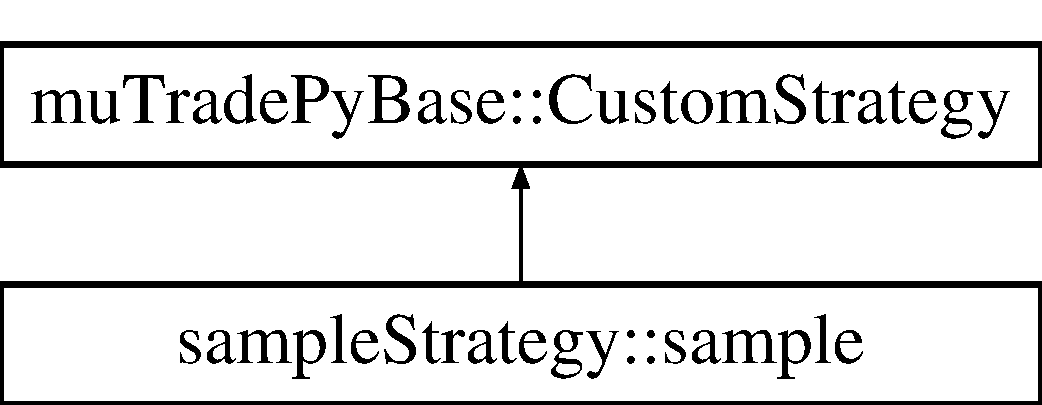
\includegraphics[height=2.000000cm]{classmuTradePyBase_1_1CustomStrategy}
\end{center}
\end{figure}
\subsection*{Public Member Functions}
\begin{DoxyCompactItemize}
\item 
def \hyperlink{classmuTradePyBase_1_1CustomStrategy_a92a6a08fb0bd5376f336bf60dbbe6152}{\-\_\-\-\_\-init\-\_\-\-\_\-}
\item 
\hypertarget{classmuTradePyBase_1_1CustomStrategy_ae8d3fbc2da91a1fcd1172e75580eeffc}{def \hyperlink{classmuTradePyBase_1_1CustomStrategy_ae8d3fbc2da91a1fcd1172e75580eeffc}{on\-Init\-Event}}\label{classmuTradePyBase_1_1CustomStrategy_ae8d3fbc2da91a1fcd1172e75580eeffc}

\begin{DoxyCompactList}\small\item\em Strategy's first event. \end{DoxyCompactList}\item 
\hypertarget{classmuTradePyBase_1_1CustomStrategy_a4c4f4e22098ac9dfaeacb5e2be97290f}{def \hyperlink{classmuTradePyBase_1_1CustomStrategy_a4c4f4e22098ac9dfaeacb5e2be97290f}{on\-C\-M\-D\-Modify\-Strategy}}\label{classmuTradePyBase_1_1CustomStrategy_a4c4f4e22098ac9dfaeacb5e2be97290f}

\begin{DoxyCompactList}\small\item\em no \end{DoxyCompactList}\item 
\hypertarget{classmuTradePyBase_1_1CustomStrategy_a9e83319de48ed28eb700dc11e961987c}{def \hyperlink{classmuTradePyBase_1_1CustomStrategy_a9e83319de48ed28eb700dc11e961987c}{on\-C\-M\-D\-Terminate\-Startegy}}\label{classmuTradePyBase_1_1CustomStrategy_a9e83319de48ed28eb700dc11e961987c}

\begin{DoxyCompactList}\small\item\em no \end{DoxyCompactList}\item 
\hypertarget{classmuTradePyBase_1_1CustomStrategy_a80d426e07d82138f4a4efd8374c3db17}{def \hyperlink{classmuTradePyBase_1_1CustomStrategy_a80d426e07d82138f4a4efd8374c3db17}{on\-C\-M\-D\-Terminate\-Sq\-Off\-Strategy}}\label{classmuTradePyBase_1_1CustomStrategy_a80d426e07d82138f4a4efd8374c3db17}

\begin{DoxyCompactList}\small\item\em no \end{DoxyCompactList}\item 
\hypertarget{classmuTradePyBase_1_1CustomStrategy_a72511bc733be7533bdc39296ed25adab}{def \hyperlink{classmuTradePyBase_1_1CustomStrategy_a72511bc733be7533bdc39296ed25adab}{on\-Default\-Event}}\label{classmuTradePyBase_1_1CustomStrategy_a72511bc733be7533bdc39296ed25adab}

\begin{DoxyCompactList}\small\item\em Default periodic event. \end{DoxyCompactList}\item 
def \hyperlink{classmuTradePyBase_1_1CustomStrategy_a918b835dffeef7990e956782842e5343}{on\-Market\-Data\-Event}
\begin{DoxyCompactList}\small\item\em Event when new market data is received. \end{DoxyCompactList}\item 
def \hyperlink{classmuTradePyBase_1_1CustomStrategy_a905f984d6323fafcc385c715441bea27}{on\-Ohlc\-Time\-Out\-Event}
\item 
def \hyperlink{classmuTradePyBase_1_1CustomStrategy_ab64f3133cb5b77c3b1d921759d5911e2}{on\-Confirmed}
\begin{DoxyCompactList}\small\item\em On confirmation of order with orderid specified in it's argument. \end{DoxyCompactList}\item 
def \hyperlink{classmuTradePyBase_1_1CustomStrategy_ad3f6cce49c42ecf283febf72fcaa5931}{on\-Replaced}
\begin{DoxyCompactList}\small\item\em When the order with unique id \-: Order\-Id gets successfully replaced. \end{DoxyCompactList}\item 
def \hyperlink{classmuTradePyBase_1_1CustomStrategy_a90185b4d9a19d02a2d6f3add49367d37}{on\-Replace\-Rejected}
\begin{DoxyCompactList}\small\item\em When request to replace order with id \-: Order\-Id is rejected due to reason specified by Error\-Code. \end{DoxyCompactList}\item 
def \hyperlink{classmuTradePyBase_1_1CustomStrategy_ae9f6ff26aefcfa95d28eb331b2636349}{on\-Cancel\-Rejected}
\begin{DoxyCompactList}\small\item\em When the request to cancel an order is rejected. \end{DoxyCompactList}\item 
def \hyperlink{classmuTradePyBase_1_1CustomStrategy_a5f62cf9ef5b4d4565a9d55ab84ba7ec5}{on\-Canceled}
\begin{DoxyCompactList}\small\item\em When order with id \-: Order\-Id gets cancelled. \end{DoxyCompactList}\item 
def \hyperlink{classmuTradePyBase_1_1CustomStrategy_a37168737333e7a2f24523729b472a923}{on\-New\-Rejected}
\begin{DoxyCompactList}\small\item\em when new placed order is rejected by the market \end{DoxyCompactList}\item 
def \hyperlink{classmuTradePyBase_1_1CustomStrategy_a925b4e45e1e2154cfe8ab4fc537fc9a6}{on\-I\-O\-C\-Canceled}
\begin{DoxyCompactList}\small\item\em When the some quantity of I\-O\-C order with id \-: Order\-Id was cancelled. \end{DoxyCompactList}\item 
def \hyperlink{classmuTradePyBase_1_1CustomStrategy_a47a2cb28592cf7c86df3bb115ca71e80}{on\-Filled}
\begin{DoxyCompactList}\small\item\em When the order with id \-: Order\-Id was completely filled. \end{DoxyCompactList}\item 
def \hyperlink{classmuTradePyBase_1_1CustomStrategy_a0f72b6e5d904bba083ef8fb40f0252f0}{on\-Partial\-Fill}
\begin{DoxyCompactList}\small\item\em When the order with id \-: Order\-Id was partially filled. \end{DoxyCompactList}\item 
def \hyperlink{classmuTradePyBase_1_1CustomStrategy_a84ad201271dca01c3753844427013726}{on\-Market\-To\-Limit}
\begin{DoxyCompactList}\small\item\em order converted from market to limit \end{DoxyCompactList}\item 
def \hyperlink{classmuTradePyBase_1_1CustomStrategy_a99f58611a2483c2015b219abdee61962}{on\-Frozen}
\begin{DoxyCompactList}\small\item\em when the order with id \-: Order\-Id gets frozen in the exchange \end{DoxyCompactList}\item 
\hypertarget{classmuTradePyBase_1_1CustomStrategy_a5dfc1f4f597d7d34962d5f7339d54e9f}{def \hyperlink{classmuTradePyBase_1_1CustomStrategy_a5dfc1f4f597d7d34962d5f7339d54e9f}{on\-Timer\-Event}}\label{classmuTradePyBase_1_1CustomStrategy_a5dfc1f4f597d7d34962d5f7339d54e9f}

\begin{DoxyCompactList}\small\item\em occurs after a periodic time interval as asked by the user \end{DoxyCompactList}\item 
def \hyperlink{classmuTradePyBase_1_1CustomStrategy_a37a7abc5e085f6eadba1e4663f144ab0}{create\-Instrument}
\begin{DoxyCompactList}\small\item\em create\-New\-Instrument To add a new Instrument in the strategy. \end{DoxyCompactList}\item 
def \hyperlink{classmuTradePyBase_1_1CustomStrategy_a8c29e9de1e8262dcc2988fa40d2760d6}{create\-Instrument\-From\-Symbol\-Format}
\begin{DoxyCompactList}\small\item\em create\-New\-Instrument To add a new Instrument in the strategy. \end{DoxyCompactList}\item 
def \hyperlink{classmuTradePyBase_1_1CustomStrategy_a55cfc91c1238c21c6fe84c3ea2fb6040}{req\-Place\-New\-Order}
\begin{DoxyCompactList}\small\item\em places a new single order \end{DoxyCompactList}\item 
def \hyperlink{classmuTradePyBase_1_1CustomStrategy_ab7410ea1556987251083ec8cd97ea9cc}{req\-Place\-Replace\-New\-Order}
\begin{DoxyCompactList}\small\item\em replaces an existing order with id \-: order\-Id by a new single order \end{DoxyCompactList}\item 
def \hyperlink{classmuTradePyBase_1_1CustomStrategy_a6f326409830d2c7a7463eed7c356f070}{req\-Place\-Cancel\-Order}
\begin{DoxyCompactList}\small\item\em cancels an existing single order with id \-: order\-Id \end{DoxyCompactList}\item 
def \hyperlink{classmuTradePyBase_1_1CustomStrategy_a0a0951d41f3700be8a501506ec802f96}{req\-Start\-Algo}
\begin{DoxyCompactList}\small\item\em function call to Start the Strategy listening to O\-H\-L\-C update events \end{DoxyCompactList}\item 
def \hyperlink{classmuTradePyBase_1_1CustomStrategy_a5c7564a367c3c88a87757cb9ed1ba524}{req\-Update\-Market\-Data}
\begin{DoxyCompactList}\small\item\em req\-Update\-Market\-Data To manually update Market Feed for all registered Instruments. \end{DoxyCompactList}\item 
def \hyperlink{classmuTradePyBase_1_1CustomStrategy_abc1635dff1eb4c69e2186fa29b4c8389}{req\-Register\-Timer\-Event}
\begin{DoxyCompactList}\small\item\em To request for a Timer-\/\-Based event, The event to be called back in time duration passed as argument in microseconds. \end{DoxyCompactList}\item 
def \hyperlink{classmuTradePyBase_1_1CustomStrategy_a337047b7b53dd750bf49d0c5d2bb3aa7}{req\-Terminate\-Strategy}
\begin{DoxyCompactList}\small\item\em req\-Terminate\-Strategy Called to Terminate Strategy. \end{DoxyCompactList}\item 
\hypertarget{classmuTradePyBase_1_1CustomStrategy_a0ee6f82eaa36ab5ee2e41ac377915c89}{def \hyperlink{classmuTradePyBase_1_1CustomStrategy_a0ee6f82eaa36ab5ee2e41ac377915c89}{req\-Terminate\-Sq\-Off\-Strategy}}\label{classmuTradePyBase_1_1CustomStrategy_a0ee6f82eaa36ab5ee2e41ac377915c89}

\begin{DoxyCompactList}\small\item\em Called to Terminate strategy and Square-\/\-Off all Positions. \end{DoxyCompactList}\item 
def \hyperlink{classmuTradePyBase_1_1CustomStrategy_a031e451622d3607fe0f99c17795d566d}{req\-Qry\-Price}
\item 
def \hyperlink{classmuTradePyBase_1_1CustomStrategy_a7ea60e547430b6610974707a3f45430d}{req\-Qry\-Qty}
\item 
def \hyperlink{classmuTradePyBase_1_1CustomStrategy_a1bd456257c3c2fdcb3ed0cd22f4c6f56}{req\-Qry\-Last\-Trade\-Price}
\item 
def \hyperlink{classmuTradePyBase_1_1CustomStrategy_ae3c193d85cc5646d9b00eedd947c7301}{req\-Qry\-Last\-Trade\-Qty}
\item 
def \hyperlink{classmuTradePyBase_1_1CustomStrategy_a43f7cda049e16a6a966c3547dd2a8b0e}{req\-Qry\-Open\-Price}
\item 
def \hyperlink{classmuTradePyBase_1_1CustomStrategy_a13df1f64c71be14f579815e938fffba2}{req\-Qry\-High\-Price}
\item 
def \hyperlink{classmuTradePyBase_1_1CustomStrategy_af73b78773ef2251fed7aa9f174fb2a76}{req\-Qry\-Low\-Price}
\item 
def \hyperlink{classmuTradePyBase_1_1CustomStrategy_a40d413bcd781c8375aa159e711902dbe}{req\-Qry\-Close\-Price}
\item 
def \hyperlink{classmuTradePyBase_1_1CustomStrategy_ab407c2c9c5a2465da0ac761d3191314b}{req\-Qry\-Volume}
\item 
def \hyperlink{classmuTradePyBase_1_1CustomStrategy_a93a925e3d1e1216103c8564eb07b9ae0}{req\-Qry\-Quote\-Last\-Update\-Time}
\item 
def \hyperlink{classmuTradePyBase_1_1CustomStrategy_ad300c984da4dfa01e2404afbb49252b3}{req\-Qry\-Instrument\-Id}
\item 
def \hyperlink{classmuTradePyBase_1_1CustomStrategy_aed341505e024c28a356bc933fdcd3d7f}{req\-Qry\-Last\-Quoted\-Price}
\item 
def \hyperlink{classmuTradePyBase_1_1CustomStrategy_aa3dea3c1de8b77262510f97841fe639c}{req\-Qry\-Open\-Qty}
\item 
def \hyperlink{classmuTradePyBase_1_1CustomStrategy_a58f6c1dc1cbad4adf97f76339ca0c349}{req\-Qry\-Traded\-Qty}
\item 
def \hyperlink{classmuTradePyBase_1_1CustomStrategy_aa378f72d5b382f297b119891feea7c24}{req\-Qry\-Open\-Side}
\item 
def \hyperlink{classmuTradePyBase_1_1CustomStrategy_a2c6a76bc23fbab884b54abd1afbcc8b0}{req\-Qry\-Booked\-Pnl}
\item 
def \hyperlink{classmuTradePyBase_1_1CustomStrategy_a65120522f9f51a39c2ea2b8bbd885fbc}{req\-Qry\-Mtm\-Pnl}
\item 
def \hyperlink{classmuTradePyBase_1_1CustomStrategy_a36ef2df689598d77b3cfa62603772a97}{req\-Qry\-Avg\-Price}
\item 
def \hyperlink{classmuTradePyBase_1_1CustomStrategy_a09404e61148b472c6bf7d99c0f99aab0}{req\-Qry\-Pending\-Qty}
\item 
def \hyperlink{classmuTradePyBase_1_1CustomStrategy_a8f4042274a3c273711bf1ff781c07523}{req\-Qry\-Client\-Id}
\item 
def \hyperlink{classmuTradePyBase_1_1CustomStrategy_a14df454fbb91052ca189cbb08716ddb0}{req\-Qry\-Net\-Booked\-P\-L}
\item 
def \hyperlink{classmuTradePyBase_1_1CustomStrategy_a0359e30c7d98026bb840550ef97f608e}{req\-Qry\-Net\-Mark\-To\-Mark\-P\-L}
\item 
def \hyperlink{classmuTradePyBase_1_1CustomStrategy_a671886bb680bfcbe5039ca1d5445bb08}{req\-Qry\-Symbol\-Id}
\item 
def \hyperlink{classmuTradePyBase_1_1CustomStrategy_a4a72dc7dbbf2ff9046052da97d364a0f}{req\-Qry\-Instrument\-List}
\begin{DoxyCompactList}\small\item\em function not available yet \end{DoxyCompactList}\item 
def \hyperlink{classmuTradePyBase_1_1CustomStrategy_a41ff84529c342931c32890b54e6b642d}{req\-Qry\-All\-Instruments}
\begin{DoxyCompactList}\small\item\em function not available yet \end{DoxyCompactList}\item 
def \hyperlink{classmuTradePyBase_1_1CustomStrategy_a69f43e16ee7fc44e44ef11f7ec45fe52}{req\-Qry\-Exchange\-Order\-Id}
\item 
def \hyperlink{classmuTradePyBase_1_1CustomStrategy_a70d6f6d5bbcd6cd8123bc4014702f193}{req\-Add\-Log\-Message}
\begin{DoxyCompactList}\small\item\em can add messages to logs \end{DoxyCompactList}\item 
\hypertarget{classmuTradePyBase_1_1CustomStrategy_abc684cd852bbd82b4445f0e142b53196}{def \hyperlink{classmuTradePyBase_1_1CustomStrategy_abc684cd852bbd82b4445f0e142b53196}{req\-Flush\-Log\-Message}}\label{classmuTradePyBase_1_1CustomStrategy_abc684cd852bbd82b4445f0e142b53196}

\begin{DoxyCompactList}\small\item\em flushes messages into a file \end{DoxyCompactList}\item 
def \hyperlink{classmuTradePyBase_1_1CustomStrategy_a783fc19776f20c4bbf45bcf1384301cf}{req\-Qry\-Strategy\-I\-D}
\item 
def \hyperlink{classmuTradePyBase_1_1CustomStrategy_a10b0158e6ee017a217f5ca781665ebf5}{req\-Qry\-Order\-Pending\-Qty}
\item 
def \hyperlink{classmuTradePyBase_1_1CustomStrategy_a406bd4255541760e42558b6d9e3ea970}{req\-Qry\-Instrument\-Pending\-Qty}
\item 
def \hyperlink{classmuTradePyBase_1_1CustomStrategy_a85b752c1b42ee6aa812486e373ae6aa7}{req\-Qry\-Client\-Order\-I\-D}
\item 
def \hyperlink{classmuTradePyBase_1_1CustomStrategy_abc3e6aa17fa14d4796ad0d69e54d0847}{req\-Qry\-Order\-Status}
\item 
def \hyperlink{classmuTradePyBase_1_1CustomStrategy_a1a44069e7158cf94df350fd83bcfcbfe}{get\-Market\-Data\-Event\-Required}
\item 
def \hyperlink{classmuTradePyBase_1_1CustomStrategy_aac6f961846182e3b427d1cb683a62777}{get\-O\-H\-L\-C\-Data\-Event\-Required}
\end{DoxyCompactItemize}
\subsection*{Public Attributes}
\begin{DoxyCompactItemize}
\item 
\hypertarget{classmuTradePyBase_1_1CustomStrategy_ae242144123c146f95fbb938e3ba7963f}{{\bfseries token\-Id}}\label{classmuTradePyBase_1_1CustomStrategy_ae242144123c146f95fbb938e3ba7963f}

\item 
\hypertarget{classmuTradePyBase_1_1CustomStrategy_a1eccd957cad582b48154287d2110cdc0}{{\bfseries f}}\label{classmuTradePyBase_1_1CustomStrategy_a1eccd957cad582b48154287d2110cdc0}

\end{DoxyCompactItemize}


\subsection{Constructor \& Destructor Documentation}
\hypertarget{classmuTradePyBase_1_1CustomStrategy_a92a6a08fb0bd5376f336bf60dbbe6152}{\index{mu\-Trade\-Py\-Base\-::\-Custom\-Strategy@{mu\-Trade\-Py\-Base\-::\-Custom\-Strategy}!\-\_\-\-\_\-init\-\_\-\-\_\-@{\-\_\-\-\_\-init\-\_\-\-\_\-}}
\index{\-\_\-\-\_\-init\-\_\-\-\_\-@{\-\_\-\-\_\-init\-\_\-\-\_\-}!muTradePyBase::CustomStrategy@{mu\-Trade\-Py\-Base\-::\-Custom\-Strategy}}
\subsubsection[{\-\_\-\-\_\-init\-\_\-\-\_\-}]{\setlength{\rightskip}{0pt plus 5cm}def mu\-Trade\-Py\-Base.\-Custom\-Strategy.\-\_\-\-\_\-init\-\_\-\-\_\- (
\begin{DoxyParamCaption}
\item[{}]{self, }
\item[{}]{token\-Id}
\end{DoxyParamCaption}
)}}\label{classmuTradePyBase_1_1CustomStrategy_a92a6a08fb0bd5376f336bf60dbbe6152}
\begin{DoxyVerb}The constructor\end{DoxyVerb}
 

\subsection{Member Function Documentation}
\hypertarget{classmuTradePyBase_1_1CustomStrategy_a37a7abc5e085f6eadba1e4663f144ab0}{\index{mu\-Trade\-Py\-Base\-::\-Custom\-Strategy@{mu\-Trade\-Py\-Base\-::\-Custom\-Strategy}!create\-Instrument@{create\-Instrument}}
\index{create\-Instrument@{create\-Instrument}!muTradePyBase::CustomStrategy@{mu\-Trade\-Py\-Base\-::\-Custom\-Strategy}}
\subsubsection[{create\-Instrument}]{\setlength{\rightskip}{0pt plus 5cm}def mu\-Trade\-Py\-Base.\-Custom\-Strategy.\-create\-Instrument (
\begin{DoxyParamCaption}
\item[{}]{self, }
\item[{}]{Instrument\-Id, }
\item[{}]{Register\-Mkt\-Data, }
\item[{}]{Use\-Snapshot, }
\item[{}]{Use\-O\-H\-C\-L}
\end{DoxyParamCaption}
)}}\label{classmuTradePyBase_1_1CustomStrategy_a37a7abc5e085f6eadba1e4663f144ab0}


create\-New\-Instrument To add a new Instrument in the strategy. 

The Pointer to the added Instrument is set in instrument passed as reference 
\begin{DoxyParams}{Parameters}
{\em symbol\-Id} & System Unique I\-D for the Instrument as A\-P\-I2\-::\-D\-A\-T\-A\-\_\-\-T\-Y\-P\-E\-S\-::\-S\-Y\-M\-B\-O\-L\-\_\-\-I\-D \\
\hline
{\em reg\-Mkt\-Data} & set True to register for Market Data for the Instrument \\
\hline
{\em use\-Snap\-Shot} & Set True if Snapshot Feed is to be used and False to use T\-B\-T-\/\-Feed \\
\hline
{\em use\-Ohlc} & Set True if O\-H\-L\-C Heed is also required \\
\hline
\end{DoxyParams}

\begin{DoxyExceptions}{Exceptions}
{\em Market\-Data\-Subscription\-Failed\-Exception} & \\
\hline
\end{DoxyExceptions}
\begin{DoxyReturn}{Returns}
C\-O\-M\-M\-O\-N\-::\-Instrument Pointer 
\end{DoxyReturn}
\hypertarget{classmuTradePyBase_1_1CustomStrategy_a8c29e9de1e8262dcc2988fa40d2760d6}{\index{mu\-Trade\-Py\-Base\-::\-Custom\-Strategy@{mu\-Trade\-Py\-Base\-::\-Custom\-Strategy}!create\-Instrument\-From\-Symbol\-Format@{create\-Instrument\-From\-Symbol\-Format}}
\index{create\-Instrument\-From\-Symbol\-Format@{create\-Instrument\-From\-Symbol\-Format}!muTradePyBase::CustomStrategy@{mu\-Trade\-Py\-Base\-::\-Custom\-Strategy}}
\subsubsection[{create\-Instrument\-From\-Symbol\-Format}]{\setlength{\rightskip}{0pt plus 5cm}def mu\-Trade\-Py\-Base.\-Custom\-Strategy.\-create\-Instrument\-From\-Symbol\-Format (
\begin{DoxyParamCaption}
\item[{}]{self, }
\item[{}]{Instrument\-Id, }
\item[{}]{Register\-Mkt\-Data, }
\item[{}]{Use\-Snapshot, }
\item[{}]{Use\-O\-H\-C\-L}
\end{DoxyParamCaption}
)}}\label{classmuTradePyBase_1_1CustomStrategy_a8c29e9de1e8262dcc2988fa40d2760d6}


create\-New\-Instrument To add a new Instrument in the strategy. 

The Pointer to the added Instrument is set in instrument passed as reference 
\begin{DoxyParams}{Parameters}
{\em instrument\-Name} & Instrument Name Format\-: \mbox{[}Exchange\-Name\mbox{]} \mbox{[}Symbol\mbox{]} \mbox{[}Expiry(\-Y\-Y\-Y\-Y\-M\-M\-D\-D)\mbox{]} \mbox{[}Strike\-Price\mbox{]} \mbox{[}C/\-P(For Call/\-Put)\mbox{]} Example\-: Cash Segment\-: N\-S\-E R\-E\-L\-I\-A\-N\-C\-E Futures Segment\-: N\-S\-E R\-E\-L\-I\-A\-N\-C\-E 20140828 Options Segment\-: N\-S\-E R\-E\-L\-I\-A\-N\-C\-E 20140828 980.\-00 C \\
\hline
{\em reg\-Mkt\-Data} & set True to register for Market Data for the Instrument \\
\hline
{\em use\-Snap\-Shot} & Set True if Snapshot Feed is to be used and False to use T\-B\-T-\/\-Feed \\
\hline
{\em use\-Ohlc} & Set True if O\-H\-L\-C Heed is also required \\
\hline
\end{DoxyParams}
\begin{DoxyReturn}{Returns}
long Instrument 
\end{DoxyReturn}

\begin{DoxyExceptions}{Exceptions}
{\em Market\-Data\-Subscription\-Failed\-Exception} & \\
\hline
\end{DoxyExceptions}
\hypertarget{classmuTradePyBase_1_1CustomStrategy_a1a44069e7158cf94df350fd83bcfcbfe}{\index{mu\-Trade\-Py\-Base\-::\-Custom\-Strategy@{mu\-Trade\-Py\-Base\-::\-Custom\-Strategy}!get\-Market\-Data\-Event\-Required@{get\-Market\-Data\-Event\-Required}}
\index{get\-Market\-Data\-Event\-Required@{get\-Market\-Data\-Event\-Required}!muTradePyBase::CustomStrategy@{mu\-Trade\-Py\-Base\-::\-Custom\-Strategy}}
\subsubsection[{get\-Market\-Data\-Event\-Required}]{\setlength{\rightskip}{0pt plus 5cm}def mu\-Trade\-Py\-Base.\-Custom\-Strategy.\-get\-Market\-Data\-Event\-Required (
\begin{DoxyParamCaption}
\item[{}]{self}
\end{DoxyParamCaption}
)}}\label{classmuTradePyBase_1_1CustomStrategy_a1a44069e7158cf94df350fd83bcfcbfe}
\begin{DoxyReturn}{Returns}
market data event flag 
\end{DoxyReturn}
\hypertarget{classmuTradePyBase_1_1CustomStrategy_aac6f961846182e3b427d1cb683a62777}{\index{mu\-Trade\-Py\-Base\-::\-Custom\-Strategy@{mu\-Trade\-Py\-Base\-::\-Custom\-Strategy}!get\-O\-H\-L\-C\-Data\-Event\-Required@{get\-O\-H\-L\-C\-Data\-Event\-Required}}
\index{get\-O\-H\-L\-C\-Data\-Event\-Required@{get\-O\-H\-L\-C\-Data\-Event\-Required}!muTradePyBase::CustomStrategy@{mu\-Trade\-Py\-Base\-::\-Custom\-Strategy}}
\subsubsection[{get\-O\-H\-L\-C\-Data\-Event\-Required}]{\setlength{\rightskip}{0pt plus 5cm}def mu\-Trade\-Py\-Base.\-Custom\-Strategy.\-get\-O\-H\-L\-C\-Data\-Event\-Required (
\begin{DoxyParamCaption}
\item[{}]{self}
\end{DoxyParamCaption}
)}}\label{classmuTradePyBase_1_1CustomStrategy_aac6f961846182e3b427d1cb683a62777}
\begin{DoxyReturn}{Returns}
O\-H\-L\-C flag 
\end{DoxyReturn}
\hypertarget{classmuTradePyBase_1_1CustomStrategy_a5f62cf9ef5b4d4565a9d55ab84ba7ec5}{\index{mu\-Trade\-Py\-Base\-::\-Custom\-Strategy@{mu\-Trade\-Py\-Base\-::\-Custom\-Strategy}!on\-Canceled@{on\-Canceled}}
\index{on\-Canceled@{on\-Canceled}!muTradePyBase::CustomStrategy@{mu\-Trade\-Py\-Base\-::\-Custom\-Strategy}}
\subsubsection[{on\-Canceled}]{\setlength{\rightskip}{0pt plus 5cm}def mu\-Trade\-Py\-Base.\-Custom\-Strategy.\-on\-Canceled (
\begin{DoxyParamCaption}
\item[{}]{self, }
\item[{}]{Order\-Id}
\end{DoxyParamCaption}
)}}\label{classmuTradePyBase_1_1CustomStrategy_a5f62cf9ef5b4d4565a9d55ab84ba7ec5}


When order with id \-: Order\-Id gets cancelled. 


\begin{DoxyParams}{Parameters}
{\em Order\-Id} & unique id of the order that was cancelled \\
\hline
\end{DoxyParams}
\hypertarget{classmuTradePyBase_1_1CustomStrategy_ae9f6ff26aefcfa95d28eb331b2636349}{\index{mu\-Trade\-Py\-Base\-::\-Custom\-Strategy@{mu\-Trade\-Py\-Base\-::\-Custom\-Strategy}!on\-Cancel\-Rejected@{on\-Cancel\-Rejected}}
\index{on\-Cancel\-Rejected@{on\-Cancel\-Rejected}!muTradePyBase::CustomStrategy@{mu\-Trade\-Py\-Base\-::\-Custom\-Strategy}}
\subsubsection[{on\-Cancel\-Rejected}]{\setlength{\rightskip}{0pt plus 5cm}def mu\-Trade\-Py\-Base.\-Custom\-Strategy.\-on\-Cancel\-Rejected (
\begin{DoxyParamCaption}
\item[{}]{self, }
\item[{}]{Order\-Id, }
\item[{}]{Error\-Code}
\end{DoxyParamCaption}
)}}\label{classmuTradePyBase_1_1CustomStrategy_ae9f6ff26aefcfa95d28eb331b2636349}


When the request to cancel an order is rejected. 


\begin{DoxyParams}{Parameters}
{\em Order\-Id} & unique id of the order to be cancelled \\
\hline
{\em Error\-Code} & reason for rejection \\
\hline
\end{DoxyParams}
\hypertarget{classmuTradePyBase_1_1CustomStrategy_ab64f3133cb5b77c3b1d921759d5911e2}{\index{mu\-Trade\-Py\-Base\-::\-Custom\-Strategy@{mu\-Trade\-Py\-Base\-::\-Custom\-Strategy}!on\-Confirmed@{on\-Confirmed}}
\index{on\-Confirmed@{on\-Confirmed}!muTradePyBase::CustomStrategy@{mu\-Trade\-Py\-Base\-::\-Custom\-Strategy}}
\subsubsection[{on\-Confirmed}]{\setlength{\rightskip}{0pt plus 5cm}def mu\-Trade\-Py\-Base.\-Custom\-Strategy.\-on\-Confirmed (
\begin{DoxyParamCaption}
\item[{}]{self, }
\item[{}]{Order\-Id}
\end{DoxyParamCaption}
)}}\label{classmuTradePyBase_1_1CustomStrategy_ab64f3133cb5b77c3b1d921759d5911e2}


On confirmation of order with orderid specified in it's argument. 


\begin{DoxyParams}{Parameters}
{\em Order\-Id} & unique id for each order placed \\
\hline
\end{DoxyParams}
\hypertarget{classmuTradePyBase_1_1CustomStrategy_a47a2cb28592cf7c86df3bb115ca71e80}{\index{mu\-Trade\-Py\-Base\-::\-Custom\-Strategy@{mu\-Trade\-Py\-Base\-::\-Custom\-Strategy}!on\-Filled@{on\-Filled}}
\index{on\-Filled@{on\-Filled}!muTradePyBase::CustomStrategy@{mu\-Trade\-Py\-Base\-::\-Custom\-Strategy}}
\subsubsection[{on\-Filled}]{\setlength{\rightskip}{0pt plus 5cm}def mu\-Trade\-Py\-Base.\-Custom\-Strategy.\-on\-Filled (
\begin{DoxyParamCaption}
\item[{}]{self, }
\item[{}]{Order\-Id, }
\item[{}]{Last\-Fill\-Price, }
\item[{}]{Last\-Fill\-Qty}
\end{DoxyParamCaption}
)}}\label{classmuTradePyBase_1_1CustomStrategy_a47a2cb28592cf7c86df3bb115ca71e80}


When the order with id \-: Order\-Id was completely filled. 


\begin{DoxyParams}{Parameters}
{\em Order\-Id} & unique id of the order that was filled \\
\hline
{\em Last\-Fill\-Price} & last price at which your order was filled \\
\hline
{\em Last\-Fill\-Qty} & the qty filled wrt Last\-Fill\-Price \\
\hline
\end{DoxyParams}
\hypertarget{classmuTradePyBase_1_1CustomStrategy_a99f58611a2483c2015b219abdee61962}{\index{mu\-Trade\-Py\-Base\-::\-Custom\-Strategy@{mu\-Trade\-Py\-Base\-::\-Custom\-Strategy}!on\-Frozen@{on\-Frozen}}
\index{on\-Frozen@{on\-Frozen}!muTradePyBase::CustomStrategy@{mu\-Trade\-Py\-Base\-::\-Custom\-Strategy}}
\subsubsection[{on\-Frozen}]{\setlength{\rightskip}{0pt plus 5cm}def mu\-Trade\-Py\-Base.\-Custom\-Strategy.\-on\-Frozen (
\begin{DoxyParamCaption}
\item[{}]{self, }
\item[{}]{Order\-Id}
\end{DoxyParamCaption}
)}}\label{classmuTradePyBase_1_1CustomStrategy_a99f58611a2483c2015b219abdee61962}


when the order with id \-: Order\-Id gets frozen in the exchange 


\begin{DoxyParams}{Parameters}
{\em Order\-Id} & id of the order which is frozen in the market \\
\hline
\end{DoxyParams}
\hypertarget{classmuTradePyBase_1_1CustomStrategy_a925b4e45e1e2154cfe8ab4fc537fc9a6}{\index{mu\-Trade\-Py\-Base\-::\-Custom\-Strategy@{mu\-Trade\-Py\-Base\-::\-Custom\-Strategy}!on\-I\-O\-C\-Canceled@{on\-I\-O\-C\-Canceled}}
\index{on\-I\-O\-C\-Canceled@{on\-I\-O\-C\-Canceled}!muTradePyBase::CustomStrategy@{mu\-Trade\-Py\-Base\-::\-Custom\-Strategy}}
\subsubsection[{on\-I\-O\-C\-Canceled}]{\setlength{\rightskip}{0pt plus 5cm}def mu\-Trade\-Py\-Base.\-Custom\-Strategy.\-on\-I\-O\-C\-Canceled (
\begin{DoxyParamCaption}
\item[{}]{self, }
\item[{}]{Order\-Id, }
\item[{}]{Canceled\-Qty}
\end{DoxyParamCaption}
)}}\label{classmuTradePyBase_1_1CustomStrategy_a925b4e45e1e2154cfe8ab4fc537fc9a6}


When the some quantity of I\-O\-C order with id \-: Order\-Id was cancelled. 


\begin{DoxyParams}{Parameters}
{\em Order\-Id} & unique id of the I\-O\-C order that was cancelled \\
\hline
{\em Canceled\-Qty} & specifies the quantity of order that was cancelled \\
\hline
\end{DoxyParams}
\hypertarget{classmuTradePyBase_1_1CustomStrategy_a918b835dffeef7990e956782842e5343}{\index{mu\-Trade\-Py\-Base\-::\-Custom\-Strategy@{mu\-Trade\-Py\-Base\-::\-Custom\-Strategy}!on\-Market\-Data\-Event@{on\-Market\-Data\-Event}}
\index{on\-Market\-Data\-Event@{on\-Market\-Data\-Event}!muTradePyBase::CustomStrategy@{mu\-Trade\-Py\-Base\-::\-Custom\-Strategy}}
\subsubsection[{on\-Market\-Data\-Event}]{\setlength{\rightskip}{0pt plus 5cm}def mu\-Trade\-Py\-Base.\-Custom\-Strategy.\-on\-Market\-Data\-Event (
\begin{DoxyParamCaption}
\item[{}]{self, }
\item[{}]{Instrument\-Id}
\end{DoxyParamCaption}
)}}\label{classmuTradePyBase_1_1CustomStrategy_a918b835dffeef7990e956782842e5343}


Event when new market data is received. 


\begin{DoxyParams}{Parameters}
{\em Instrument\-Id} & symbolic representation of the instrument being traded \\
\hline
\end{DoxyParams}
\hypertarget{classmuTradePyBase_1_1CustomStrategy_a84ad201271dca01c3753844427013726}{\index{mu\-Trade\-Py\-Base\-::\-Custom\-Strategy@{mu\-Trade\-Py\-Base\-::\-Custom\-Strategy}!on\-Market\-To\-Limit@{on\-Market\-To\-Limit}}
\index{on\-Market\-To\-Limit@{on\-Market\-To\-Limit}!muTradePyBase::CustomStrategy@{mu\-Trade\-Py\-Base\-::\-Custom\-Strategy}}
\subsubsection[{on\-Market\-To\-Limit}]{\setlength{\rightskip}{0pt plus 5cm}def mu\-Trade\-Py\-Base.\-Custom\-Strategy.\-on\-Market\-To\-Limit (
\begin{DoxyParamCaption}
\item[{}]{self, }
\item[{}]{Order\-Id}
\end{DoxyParamCaption}
)}}\label{classmuTradePyBase_1_1CustomStrategy_a84ad201271dca01c3753844427013726}


order converted from market to limit 


\begin{DoxyParams}{Parameters}
{\em Order\-Id} & id of the order converted \\
\hline
\end{DoxyParams}
\hypertarget{classmuTradePyBase_1_1CustomStrategy_a37168737333e7a2f24523729b472a923}{\index{mu\-Trade\-Py\-Base\-::\-Custom\-Strategy@{mu\-Trade\-Py\-Base\-::\-Custom\-Strategy}!on\-New\-Rejected@{on\-New\-Rejected}}
\index{on\-New\-Rejected@{on\-New\-Rejected}!muTradePyBase::CustomStrategy@{mu\-Trade\-Py\-Base\-::\-Custom\-Strategy}}
\subsubsection[{on\-New\-Rejected}]{\setlength{\rightskip}{0pt plus 5cm}def mu\-Trade\-Py\-Base.\-Custom\-Strategy.\-on\-New\-Rejected (
\begin{DoxyParamCaption}
\item[{}]{self, }
\item[{}]{Order\-Id, }
\item[{}]{Error\-Code}
\end{DoxyParamCaption}
)}}\label{classmuTradePyBase_1_1CustomStrategy_a37168737333e7a2f24523729b472a923}


when new placed order is rejected by the market 


\begin{DoxyParams}{Parameters}
{\em Order\-Id} & id of the new order rejected \\
\hline
{\em Error\-Code} & reason of the rejection \\
\hline
\end{DoxyParams}
\hypertarget{classmuTradePyBase_1_1CustomStrategy_a905f984d6323fafcc385c715441bea27}{\index{mu\-Trade\-Py\-Base\-::\-Custom\-Strategy@{mu\-Trade\-Py\-Base\-::\-Custom\-Strategy}!on\-Ohlc\-Time\-Out\-Event@{on\-Ohlc\-Time\-Out\-Event}}
\index{on\-Ohlc\-Time\-Out\-Event@{on\-Ohlc\-Time\-Out\-Event}!muTradePyBase::CustomStrategy@{mu\-Trade\-Py\-Base\-::\-Custom\-Strategy}}
\subsubsection[{on\-Ohlc\-Time\-Out\-Event}]{\setlength{\rightskip}{0pt plus 5cm}def mu\-Trade\-Py\-Base.\-Custom\-Strategy.\-on\-Ohlc\-Time\-Out\-Event (
\begin{DoxyParamCaption}
\item[{}]{self}
\end{DoxyParamCaption}
)}}\label{classmuTradePyBase_1_1CustomStrategy_a905f984d6323fafcc385c715441bea27}
\begin{DoxyVerb}\end{DoxyVerb}
 \hypertarget{classmuTradePyBase_1_1CustomStrategy_a0f72b6e5d904bba083ef8fb40f0252f0}{\index{mu\-Trade\-Py\-Base\-::\-Custom\-Strategy@{mu\-Trade\-Py\-Base\-::\-Custom\-Strategy}!on\-Partial\-Fill@{on\-Partial\-Fill}}
\index{on\-Partial\-Fill@{on\-Partial\-Fill}!muTradePyBase::CustomStrategy@{mu\-Trade\-Py\-Base\-::\-Custom\-Strategy}}
\subsubsection[{on\-Partial\-Fill}]{\setlength{\rightskip}{0pt plus 5cm}def mu\-Trade\-Py\-Base.\-Custom\-Strategy.\-on\-Partial\-Fill (
\begin{DoxyParamCaption}
\item[{}]{self, }
\item[{}]{Order\-Id, }
\item[{}]{Last\-Fill\-Price, }
\item[{}]{Last\-Fill\-Qty}
\end{DoxyParamCaption}
)}}\label{classmuTradePyBase_1_1CustomStrategy_a0f72b6e5d904bba083ef8fb40f0252f0}


When the order with id \-: Order\-Id was partially filled. 


\begin{DoxyParams}{Parameters}
{\em Order\-Id} & unique id of the order partially filled \\
\hline
{\em Last\-Fill\-Price} & last price at which your order was filled \\
\hline
{\em Last\-Fill\-Qty} & the qty filled wrt Last\-Fill\-Price \\
\hline
\end{DoxyParams}
\hypertarget{classmuTradePyBase_1_1CustomStrategy_ad3f6cce49c42ecf283febf72fcaa5931}{\index{mu\-Trade\-Py\-Base\-::\-Custom\-Strategy@{mu\-Trade\-Py\-Base\-::\-Custom\-Strategy}!on\-Replaced@{on\-Replaced}}
\index{on\-Replaced@{on\-Replaced}!muTradePyBase::CustomStrategy@{mu\-Trade\-Py\-Base\-::\-Custom\-Strategy}}
\subsubsection[{on\-Replaced}]{\setlength{\rightskip}{0pt plus 5cm}def mu\-Trade\-Py\-Base.\-Custom\-Strategy.\-on\-Replaced (
\begin{DoxyParamCaption}
\item[{}]{self, }
\item[{}]{Order\-Id}
\end{DoxyParamCaption}
)}}\label{classmuTradePyBase_1_1CustomStrategy_ad3f6cce49c42ecf283febf72fcaa5931}


When the order with unique id \-: Order\-Id gets successfully replaced. 


\begin{DoxyParams}{Parameters}
{\em Order\-Id} & unique id of the order replaced \\
\hline
\end{DoxyParams}
\hypertarget{classmuTradePyBase_1_1CustomStrategy_a90185b4d9a19d02a2d6f3add49367d37}{\index{mu\-Trade\-Py\-Base\-::\-Custom\-Strategy@{mu\-Trade\-Py\-Base\-::\-Custom\-Strategy}!on\-Replace\-Rejected@{on\-Replace\-Rejected}}
\index{on\-Replace\-Rejected@{on\-Replace\-Rejected}!muTradePyBase::CustomStrategy@{mu\-Trade\-Py\-Base\-::\-Custom\-Strategy}}
\subsubsection[{on\-Replace\-Rejected}]{\setlength{\rightskip}{0pt plus 5cm}def mu\-Trade\-Py\-Base.\-Custom\-Strategy.\-on\-Replace\-Rejected (
\begin{DoxyParamCaption}
\item[{}]{self, }
\item[{}]{Order\-Id, }
\item[{}]{Error\-Code}
\end{DoxyParamCaption}
)}}\label{classmuTradePyBase_1_1CustomStrategy_a90185b4d9a19d02a2d6f3add49367d37}


When request to replace order with id \-: Order\-Id is rejected due to reason specified by Error\-Code. 


\begin{DoxyParams}{Parameters}
{\em Order\-Id} & unique id of the order which was not replaced \\
\hline
{\em Error\-Code} & reason for rejection \\
\hline
\end{DoxyParams}
\hypertarget{classmuTradePyBase_1_1CustomStrategy_a70d6f6d5bbcd6cd8123bc4014702f193}{\index{mu\-Trade\-Py\-Base\-::\-Custom\-Strategy@{mu\-Trade\-Py\-Base\-::\-Custom\-Strategy}!req\-Add\-Log\-Message@{req\-Add\-Log\-Message}}
\index{req\-Add\-Log\-Message@{req\-Add\-Log\-Message}!muTradePyBase::CustomStrategy@{mu\-Trade\-Py\-Base\-::\-Custom\-Strategy}}
\subsubsection[{req\-Add\-Log\-Message}]{\setlength{\rightskip}{0pt plus 5cm}def mu\-Trade\-Py\-Base.\-Custom\-Strategy.\-req\-Add\-Log\-Message (
\begin{DoxyParamCaption}
\item[{}]{self, }
\item[{}]{message}
\end{DoxyParamCaption}
)}}\label{classmuTradePyBase_1_1CustomStrategy_a70d6f6d5bbcd6cd8123bc4014702f193}


can add messages to logs 


\begin{DoxyParams}{Parameters}
{\em message} & message you want to add to logs \\
\hline
\end{DoxyParams}
\hypertarget{classmuTradePyBase_1_1CustomStrategy_a6f326409830d2c7a7463eed7c356f070}{\index{mu\-Trade\-Py\-Base\-::\-Custom\-Strategy@{mu\-Trade\-Py\-Base\-::\-Custom\-Strategy}!req\-Place\-Cancel\-Order@{req\-Place\-Cancel\-Order}}
\index{req\-Place\-Cancel\-Order@{req\-Place\-Cancel\-Order}!muTradePyBase::CustomStrategy@{mu\-Trade\-Py\-Base\-::\-Custom\-Strategy}}
\subsubsection[{req\-Place\-Cancel\-Order}]{\setlength{\rightskip}{0pt plus 5cm}def mu\-Trade\-Py\-Base.\-Custom\-Strategy.\-req\-Place\-Cancel\-Order (
\begin{DoxyParamCaption}
\item[{}]{self, }
\item[{}]{order\-Id, }
\item[{}]{single\-Order}
\end{DoxyParamCaption}
)}}\label{classmuTradePyBase_1_1CustomStrategy_a6f326409830d2c7a7463eed7c356f070}


cancels an existing single order with id \-: order\-Id 


\begin{DoxyParams}{Parameters}
{\em order\-Id} & id of the order to be canceled \\
\hline
{\em Single\-Order} & single order to be canceled \\
\hline
\end{DoxyParams}
\begin{DoxyReturn}{Returns}
order reply object 
\end{DoxyReturn}
\hypertarget{classmuTradePyBase_1_1CustomStrategy_a55cfc91c1238c21c6fe84c3ea2fb6040}{\index{mu\-Trade\-Py\-Base\-::\-Custom\-Strategy@{mu\-Trade\-Py\-Base\-::\-Custom\-Strategy}!req\-Place\-New\-Order@{req\-Place\-New\-Order}}
\index{req\-Place\-New\-Order@{req\-Place\-New\-Order}!muTradePyBase::CustomStrategy@{mu\-Trade\-Py\-Base\-::\-Custom\-Strategy}}
\subsubsection[{req\-Place\-New\-Order}]{\setlength{\rightskip}{0pt plus 5cm}def mu\-Trade\-Py\-Base.\-Custom\-Strategy.\-req\-Place\-New\-Order (
\begin{DoxyParamCaption}
\item[{}]{self, }
\item[{}]{single\-Order}
\end{DoxyParamCaption}
)}}\label{classmuTradePyBase_1_1CustomStrategy_a55cfc91c1238c21c6fe84c3ea2fb6040}


places a new single order 


\begin{DoxyParams}{Parameters}
{\em Single\-Order} & single order object \\
\hline
\end{DoxyParams}
\begin{DoxyReturn}{Returns}
order reply object 
\end{DoxyReturn}
\hypertarget{classmuTradePyBase_1_1CustomStrategy_ab7410ea1556987251083ec8cd97ea9cc}{\index{mu\-Trade\-Py\-Base\-::\-Custom\-Strategy@{mu\-Trade\-Py\-Base\-::\-Custom\-Strategy}!req\-Place\-Replace\-New\-Order@{req\-Place\-Replace\-New\-Order}}
\index{req\-Place\-Replace\-New\-Order@{req\-Place\-Replace\-New\-Order}!muTradePyBase::CustomStrategy@{mu\-Trade\-Py\-Base\-::\-Custom\-Strategy}}
\subsubsection[{req\-Place\-Replace\-New\-Order}]{\setlength{\rightskip}{0pt plus 5cm}def mu\-Trade\-Py\-Base.\-Custom\-Strategy.\-req\-Place\-Replace\-New\-Order (
\begin{DoxyParamCaption}
\item[{}]{self, }
\item[{}]{order\-Id, }
\item[{}]{single\-Order}
\end{DoxyParamCaption}
)}}\label{classmuTradePyBase_1_1CustomStrategy_ab7410ea1556987251083ec8cd97ea9cc}


replaces an existing order with id \-: order\-Id by a new single order 


\begin{DoxyParams}{Parameters}
{\em order\-Id} & id of the order to be replaced \\
\hline
{\em Single\-Order} & single order object \\
\hline
\end{DoxyParams}
\begin{DoxyReturn}{Returns}
order reply object 
\end{DoxyReturn}
\hypertarget{classmuTradePyBase_1_1CustomStrategy_a41ff84529c342931c32890b54e6b642d}{\index{mu\-Trade\-Py\-Base\-::\-Custom\-Strategy@{mu\-Trade\-Py\-Base\-::\-Custom\-Strategy}!req\-Qry\-All\-Instruments@{req\-Qry\-All\-Instruments}}
\index{req\-Qry\-All\-Instruments@{req\-Qry\-All\-Instruments}!muTradePyBase::CustomStrategy@{mu\-Trade\-Py\-Base\-::\-Custom\-Strategy}}
\subsubsection[{req\-Qry\-All\-Instruments}]{\setlength{\rightskip}{0pt plus 5cm}def mu\-Trade\-Py\-Base.\-Custom\-Strategy.\-req\-Qry\-All\-Instruments (
\begin{DoxyParamCaption}
\item[{}]{self}
\end{DoxyParamCaption}
)}}\label{classmuTradePyBase_1_1CustomStrategy_a41ff84529c342931c32890b54e6b642d}


function not available yet 

\begin{DoxyReturn}{Returns}
all instruments irrespective of instrument id 
\end{DoxyReturn}
\hypertarget{classmuTradePyBase_1_1CustomStrategy_a36ef2df689598d77b3cfa62603772a97}{\index{mu\-Trade\-Py\-Base\-::\-Custom\-Strategy@{mu\-Trade\-Py\-Base\-::\-Custom\-Strategy}!req\-Qry\-Avg\-Price@{req\-Qry\-Avg\-Price}}
\index{req\-Qry\-Avg\-Price@{req\-Qry\-Avg\-Price}!muTradePyBase::CustomStrategy@{mu\-Trade\-Py\-Base\-::\-Custom\-Strategy}}
\subsubsection[{req\-Qry\-Avg\-Price}]{\setlength{\rightskip}{0pt plus 5cm}def mu\-Trade\-Py\-Base.\-Custom\-Strategy.\-req\-Qry\-Avg\-Price (
\begin{DoxyParamCaption}
\item[{}]{self, }
\item[{}]{Instrument, }
\item[{}]{mode}
\end{DoxyParamCaption}
)}}\label{classmuTradePyBase_1_1CustomStrategy_a36ef2df689598d77b3cfa62603772a97}

\begin{DoxyParams}{Parameters}
{\em Instrument} & instrument for which you need the average price \\
\hline
\end{DoxyParams}
\begin{DoxyReturn}{Returns}
average price for the respective instrument 
\end{DoxyReturn}
\hypertarget{classmuTradePyBase_1_1CustomStrategy_a2c6a76bc23fbab884b54abd1afbcc8b0}{\index{mu\-Trade\-Py\-Base\-::\-Custom\-Strategy@{mu\-Trade\-Py\-Base\-::\-Custom\-Strategy}!req\-Qry\-Booked\-Pnl@{req\-Qry\-Booked\-Pnl}}
\index{req\-Qry\-Booked\-Pnl@{req\-Qry\-Booked\-Pnl}!muTradePyBase::CustomStrategy@{mu\-Trade\-Py\-Base\-::\-Custom\-Strategy}}
\subsubsection[{req\-Qry\-Booked\-Pnl}]{\setlength{\rightskip}{0pt plus 5cm}def mu\-Trade\-Py\-Base.\-Custom\-Strategy.\-req\-Qry\-Booked\-Pnl (
\begin{DoxyParamCaption}
\item[{}]{self, }
\item[{}]{Instrument}
\end{DoxyParamCaption}
)}}\label{classmuTradePyBase_1_1CustomStrategy_a2c6a76bc23fbab884b54abd1afbcc8b0}

\begin{DoxyParams}{Parameters}
{\em Instrument} & instrument for which you need the booked pnl \\
\hline
\end{DoxyParams}
\begin{DoxyReturn}{Returns}
booked pnl for the respective instrument 
\end{DoxyReturn}
\hypertarget{classmuTradePyBase_1_1CustomStrategy_a8f4042274a3c273711bf1ff781c07523}{\index{mu\-Trade\-Py\-Base\-::\-Custom\-Strategy@{mu\-Trade\-Py\-Base\-::\-Custom\-Strategy}!req\-Qry\-Client\-Id@{req\-Qry\-Client\-Id}}
\index{req\-Qry\-Client\-Id@{req\-Qry\-Client\-Id}!muTradePyBase::CustomStrategy@{mu\-Trade\-Py\-Base\-::\-Custom\-Strategy}}
\subsubsection[{req\-Qry\-Client\-Id}]{\setlength{\rightskip}{0pt plus 5cm}def mu\-Trade\-Py\-Base.\-Custom\-Strategy.\-req\-Qry\-Client\-Id (
\begin{DoxyParamCaption}
\item[{}]{self}
\end{DoxyParamCaption}
)}}\label{classmuTradePyBase_1_1CustomStrategy_a8f4042274a3c273711bf1ff781c07523}
\begin{DoxyReturn}{Returns}
clientid 
\end{DoxyReturn}
\hypertarget{classmuTradePyBase_1_1CustomStrategy_a85b752c1b42ee6aa812486e373ae6aa7}{\index{mu\-Trade\-Py\-Base\-::\-Custom\-Strategy@{mu\-Trade\-Py\-Base\-::\-Custom\-Strategy}!req\-Qry\-Client\-Order\-I\-D@{req\-Qry\-Client\-Order\-I\-D}}
\index{req\-Qry\-Client\-Order\-I\-D@{req\-Qry\-Client\-Order\-I\-D}!muTradePyBase::CustomStrategy@{mu\-Trade\-Py\-Base\-::\-Custom\-Strategy}}
\subsubsection[{req\-Qry\-Client\-Order\-I\-D}]{\setlength{\rightskip}{0pt plus 5cm}def mu\-Trade\-Py\-Base.\-Custom\-Strategy.\-req\-Qry\-Client\-Order\-I\-D (
\begin{DoxyParamCaption}
\item[{}]{self, }
\item[{}]{order\-Id}
\end{DoxyParamCaption}
)}}\label{classmuTradePyBase_1_1CustomStrategy_a85b752c1b42ee6aa812486e373ae6aa7}

\begin{DoxyParams}{Parameters}
{\em orderid} & id of the order you want clientorderid for \\
\hline
\end{DoxyParams}
\begin{DoxyReturn}{Returns}
clientorderid corresponding to the order\-Id 
\end{DoxyReturn}
\hypertarget{classmuTradePyBase_1_1CustomStrategy_a40d413bcd781c8375aa159e711902dbe}{\index{mu\-Trade\-Py\-Base\-::\-Custom\-Strategy@{mu\-Trade\-Py\-Base\-::\-Custom\-Strategy}!req\-Qry\-Close\-Price@{req\-Qry\-Close\-Price}}
\index{req\-Qry\-Close\-Price@{req\-Qry\-Close\-Price}!muTradePyBase::CustomStrategy@{mu\-Trade\-Py\-Base\-::\-Custom\-Strategy}}
\subsubsection[{req\-Qry\-Close\-Price}]{\setlength{\rightskip}{0pt plus 5cm}def mu\-Trade\-Py\-Base.\-Custom\-Strategy.\-req\-Qry\-Close\-Price (
\begin{DoxyParamCaption}
\item[{}]{self, }
\item[{}]{Instrument\-Id}
\end{DoxyParamCaption}
)}}\label{classmuTradePyBase_1_1CustomStrategy_a40d413bcd781c8375aa159e711902dbe}

\begin{DoxyParams}{Parameters}
{\em Instrument\-Id} & Instrument\-Id of the Instrument you want the close price for \\
\hline
\end{DoxyParams}
\begin{DoxyReturn}{Returns}
close price of the instrument specified by the instrumentid 
\end{DoxyReturn}
\hypertarget{classmuTradePyBase_1_1CustomStrategy_a69f43e16ee7fc44e44ef11f7ec45fe52}{\index{mu\-Trade\-Py\-Base\-::\-Custom\-Strategy@{mu\-Trade\-Py\-Base\-::\-Custom\-Strategy}!req\-Qry\-Exchange\-Order\-Id@{req\-Qry\-Exchange\-Order\-Id}}
\index{req\-Qry\-Exchange\-Order\-Id@{req\-Qry\-Exchange\-Order\-Id}!muTradePyBase::CustomStrategy@{mu\-Trade\-Py\-Base\-::\-Custom\-Strategy}}
\subsubsection[{req\-Qry\-Exchange\-Order\-Id}]{\setlength{\rightskip}{0pt plus 5cm}def mu\-Trade\-Py\-Base.\-Custom\-Strategy.\-req\-Qry\-Exchange\-Order\-Id (
\begin{DoxyParamCaption}
\item[{}]{self, }
\item[{}]{order\-Id}
\end{DoxyParamCaption}
)}}\label{classmuTradePyBase_1_1CustomStrategy_a69f43e16ee7fc44e44ef11f7ec45fe52}

\begin{DoxyParams}{Parameters}
{\em order\-Id} & unique id of the order you want the exchange order id for \\
\hline
\end{DoxyParams}
\begin{DoxyReturn}{Returns}
exchangeorderid corresponding to the order\-Id 
\end{DoxyReturn}
\hypertarget{classmuTradePyBase_1_1CustomStrategy_a13df1f64c71be14f579815e938fffba2}{\index{mu\-Trade\-Py\-Base\-::\-Custom\-Strategy@{mu\-Trade\-Py\-Base\-::\-Custom\-Strategy}!req\-Qry\-High\-Price@{req\-Qry\-High\-Price}}
\index{req\-Qry\-High\-Price@{req\-Qry\-High\-Price}!muTradePyBase::CustomStrategy@{mu\-Trade\-Py\-Base\-::\-Custom\-Strategy}}
\subsubsection[{req\-Qry\-High\-Price}]{\setlength{\rightskip}{0pt plus 5cm}def mu\-Trade\-Py\-Base.\-Custom\-Strategy.\-req\-Qry\-High\-Price (
\begin{DoxyParamCaption}
\item[{}]{self, }
\item[{}]{Instrument\-Id}
\end{DoxyParamCaption}
)}}\label{classmuTradePyBase_1_1CustomStrategy_a13df1f64c71be14f579815e938fffba2}

\begin{DoxyParams}{Parameters}
{\em Instrument\-Id} & Instrument\-Id of the Instrument you want the high price for \\
\hline
\end{DoxyParams}
\begin{DoxyReturn}{Returns}
high price of the instrument specified by the instrumentid 
\end{DoxyReturn}
\hypertarget{classmuTradePyBase_1_1CustomStrategy_ad300c984da4dfa01e2404afbb49252b3}{\index{mu\-Trade\-Py\-Base\-::\-Custom\-Strategy@{mu\-Trade\-Py\-Base\-::\-Custom\-Strategy}!req\-Qry\-Instrument\-Id@{req\-Qry\-Instrument\-Id}}
\index{req\-Qry\-Instrument\-Id@{req\-Qry\-Instrument\-Id}!muTradePyBase::CustomStrategy@{mu\-Trade\-Py\-Base\-::\-Custom\-Strategy}}
\subsubsection[{req\-Qry\-Instrument\-Id}]{\setlength{\rightskip}{0pt plus 5cm}def mu\-Trade\-Py\-Base.\-Custom\-Strategy.\-req\-Qry\-Instrument\-Id (
\begin{DoxyParamCaption}
\item[{}]{self, }
\item[{}]{Instrument}
\end{DoxyParamCaption}
)}}\label{classmuTradePyBase_1_1CustomStrategy_ad300c984da4dfa01e2404afbb49252b3}

\begin{DoxyParams}{Parameters}
{\em Instrument} & instrument you want the instrument id for \\
\hline
\end{DoxyParams}
\begin{DoxyReturn}{Returns}
instrumentid of the corresponding instrument 
\end{DoxyReturn}
\hypertarget{classmuTradePyBase_1_1CustomStrategy_a4a72dc7dbbf2ff9046052da97d364a0f}{\index{mu\-Trade\-Py\-Base\-::\-Custom\-Strategy@{mu\-Trade\-Py\-Base\-::\-Custom\-Strategy}!req\-Qry\-Instrument\-List@{req\-Qry\-Instrument\-List}}
\index{req\-Qry\-Instrument\-List@{req\-Qry\-Instrument\-List}!muTradePyBase::CustomStrategy@{mu\-Trade\-Py\-Base\-::\-Custom\-Strategy}}
\subsubsection[{req\-Qry\-Instrument\-List}]{\setlength{\rightskip}{0pt plus 5cm}def mu\-Trade\-Py\-Base.\-Custom\-Strategy.\-req\-Qry\-Instrument\-List (
\begin{DoxyParamCaption}
\item[{}]{self, }
\item[{}]{Instrument\-Id}
\end{DoxyParamCaption}
)}}\label{classmuTradePyBase_1_1CustomStrategy_a4a72dc7dbbf2ff9046052da97d364a0f}


function not available yet 


\begin{DoxyParams}{Parameters}
{\em Instrument\-Id} & instrumentid you want all instruments for \\
\hline
\end{DoxyParams}
\begin{DoxyReturn}{Returns}
list from Instrument\-Id 
\end{DoxyReturn}
\hypertarget{classmuTradePyBase_1_1CustomStrategy_a406bd4255541760e42558b6d9e3ea970}{\index{mu\-Trade\-Py\-Base\-::\-Custom\-Strategy@{mu\-Trade\-Py\-Base\-::\-Custom\-Strategy}!req\-Qry\-Instrument\-Pending\-Qty@{req\-Qry\-Instrument\-Pending\-Qty}}
\index{req\-Qry\-Instrument\-Pending\-Qty@{req\-Qry\-Instrument\-Pending\-Qty}!muTradePyBase::CustomStrategy@{mu\-Trade\-Py\-Base\-::\-Custom\-Strategy}}
\subsubsection[{req\-Qry\-Instrument\-Pending\-Qty}]{\setlength{\rightskip}{0pt plus 5cm}def mu\-Trade\-Py\-Base.\-Custom\-Strategy.\-req\-Qry\-Instrument\-Pending\-Qty (
\begin{DoxyParamCaption}
\item[{}]{self, }
\item[{}]{Instrument, }
\item[{}]{side}
\end{DoxyParamCaption}
)}}\label{classmuTradePyBase_1_1CustomStrategy_a406bd4255541760e42558b6d9e3ea970}

\begin{DoxyParams}{Parameters}
{\em Instrument} & instrument you want pending quantity for \\
\hline
{\em side} & buy or sell \\
\hline
\end{DoxyParams}
\begin{DoxyReturn}{Returns}
pending quantity for an instrument of a particular side 
\end{DoxyReturn}
\hypertarget{classmuTradePyBase_1_1CustomStrategy_aed341505e024c28a356bc933fdcd3d7f}{\index{mu\-Trade\-Py\-Base\-::\-Custom\-Strategy@{mu\-Trade\-Py\-Base\-::\-Custom\-Strategy}!req\-Qry\-Last\-Quoted\-Price@{req\-Qry\-Last\-Quoted\-Price}}
\index{req\-Qry\-Last\-Quoted\-Price@{req\-Qry\-Last\-Quoted\-Price}!muTradePyBase::CustomStrategy@{mu\-Trade\-Py\-Base\-::\-Custom\-Strategy}}
\subsubsection[{req\-Qry\-Last\-Quoted\-Price}]{\setlength{\rightskip}{0pt plus 5cm}def mu\-Trade\-Py\-Base.\-Custom\-Strategy.\-req\-Qry\-Last\-Quoted\-Price (
\begin{DoxyParamCaption}
\item[{}]{self, }
\item[{}]{Instrument, }
\item[{}]{mode}
\end{DoxyParamCaption}
)}}\label{classmuTradePyBase_1_1CustomStrategy_aed341505e024c28a356bc933fdcd3d7f}

\begin{DoxyParams}{Parameters}
{\em Instrument\-Id} & Instrument\-Id of the Instrument you want the last update time for \\
\hline
\end{DoxyParams}
\begin{DoxyReturn}{Returns}
last update time of the instrument specified by the instrumentid 
\end{DoxyReturn}
\hypertarget{classmuTradePyBase_1_1CustomStrategy_a1bd456257c3c2fdcb3ed0cd22f4c6f56}{\index{mu\-Trade\-Py\-Base\-::\-Custom\-Strategy@{mu\-Trade\-Py\-Base\-::\-Custom\-Strategy}!req\-Qry\-Last\-Trade\-Price@{req\-Qry\-Last\-Trade\-Price}}
\index{req\-Qry\-Last\-Trade\-Price@{req\-Qry\-Last\-Trade\-Price}!muTradePyBase::CustomStrategy@{mu\-Trade\-Py\-Base\-::\-Custom\-Strategy}}
\subsubsection[{req\-Qry\-Last\-Trade\-Price}]{\setlength{\rightskip}{0pt plus 5cm}def mu\-Trade\-Py\-Base.\-Custom\-Strategy.\-req\-Qry\-Last\-Trade\-Price (
\begin{DoxyParamCaption}
\item[{}]{self, }
\item[{}]{Instrument\-Id}
\end{DoxyParamCaption}
)}}\label{classmuTradePyBase_1_1CustomStrategy_a1bd456257c3c2fdcb3ed0cd22f4c6f56}

\begin{DoxyParams}{Parameters}
{\em Instrument\-Id} & Instrument\-Id of the Instrument you want the ltp for \\
\hline
\end{DoxyParams}
\begin{DoxyReturn}{Returns}
last traded price of the instrument specified by the instrumentid 
\end{DoxyReturn}
\hypertarget{classmuTradePyBase_1_1CustomStrategy_ae3c193d85cc5646d9b00eedd947c7301}{\index{mu\-Trade\-Py\-Base\-::\-Custom\-Strategy@{mu\-Trade\-Py\-Base\-::\-Custom\-Strategy}!req\-Qry\-Last\-Trade\-Qty@{req\-Qry\-Last\-Trade\-Qty}}
\index{req\-Qry\-Last\-Trade\-Qty@{req\-Qry\-Last\-Trade\-Qty}!muTradePyBase::CustomStrategy@{mu\-Trade\-Py\-Base\-::\-Custom\-Strategy}}
\subsubsection[{req\-Qry\-Last\-Trade\-Qty}]{\setlength{\rightskip}{0pt plus 5cm}def mu\-Trade\-Py\-Base.\-Custom\-Strategy.\-req\-Qry\-Last\-Trade\-Qty (
\begin{DoxyParamCaption}
\item[{}]{self, }
\item[{}]{Instrument\-Id}
\end{DoxyParamCaption}
)}}\label{classmuTradePyBase_1_1CustomStrategy_ae3c193d85cc5646d9b00eedd947c7301}

\begin{DoxyParams}{Parameters}
{\em Instrument\-Id} & Instrument\-Id of the Instrument you want the last traded quantity for \\
\hline
\end{DoxyParams}
\begin{DoxyReturn}{Returns}
last traded quantity of the instrument specified by the instrumentid 
\end{DoxyReturn}
\hypertarget{classmuTradePyBase_1_1CustomStrategy_af73b78773ef2251fed7aa9f174fb2a76}{\index{mu\-Trade\-Py\-Base\-::\-Custom\-Strategy@{mu\-Trade\-Py\-Base\-::\-Custom\-Strategy}!req\-Qry\-Low\-Price@{req\-Qry\-Low\-Price}}
\index{req\-Qry\-Low\-Price@{req\-Qry\-Low\-Price}!muTradePyBase::CustomStrategy@{mu\-Trade\-Py\-Base\-::\-Custom\-Strategy}}
\subsubsection[{req\-Qry\-Low\-Price}]{\setlength{\rightskip}{0pt plus 5cm}def mu\-Trade\-Py\-Base.\-Custom\-Strategy.\-req\-Qry\-Low\-Price (
\begin{DoxyParamCaption}
\item[{}]{self, }
\item[{}]{Instrument\-Id}
\end{DoxyParamCaption}
)}}\label{classmuTradePyBase_1_1CustomStrategy_af73b78773ef2251fed7aa9f174fb2a76}

\begin{DoxyParams}{Parameters}
{\em Instrument\-Id} & Instrument\-Id of the Instrument you want the low price for \\
\hline
\end{DoxyParams}
\begin{DoxyReturn}{Returns}
low price of the instrument specified by the instrumentid 
\end{DoxyReturn}
\hypertarget{classmuTradePyBase_1_1CustomStrategy_a65120522f9f51a39c2ea2b8bbd885fbc}{\index{mu\-Trade\-Py\-Base\-::\-Custom\-Strategy@{mu\-Trade\-Py\-Base\-::\-Custom\-Strategy}!req\-Qry\-Mtm\-Pnl@{req\-Qry\-Mtm\-Pnl}}
\index{req\-Qry\-Mtm\-Pnl@{req\-Qry\-Mtm\-Pnl}!muTradePyBase::CustomStrategy@{mu\-Trade\-Py\-Base\-::\-Custom\-Strategy}}
\subsubsection[{req\-Qry\-Mtm\-Pnl}]{\setlength{\rightskip}{0pt plus 5cm}def mu\-Trade\-Py\-Base.\-Custom\-Strategy.\-req\-Qry\-Mtm\-Pnl (
\begin{DoxyParamCaption}
\item[{}]{self, }
\item[{}]{Instrument}
\end{DoxyParamCaption}
)}}\label{classmuTradePyBase_1_1CustomStrategy_a65120522f9f51a39c2ea2b8bbd885fbc}

\begin{DoxyParams}{Parameters}
{\em Instrument} & instrument for which you need the mtm pnl \\
\hline
\end{DoxyParams}
\begin{DoxyReturn}{Returns}
mtm pnl for the respective instrument 
\end{DoxyReturn}
\hypertarget{classmuTradePyBase_1_1CustomStrategy_a14df454fbb91052ca189cbb08716ddb0}{\index{mu\-Trade\-Py\-Base\-::\-Custom\-Strategy@{mu\-Trade\-Py\-Base\-::\-Custom\-Strategy}!req\-Qry\-Net\-Booked\-P\-L@{req\-Qry\-Net\-Booked\-P\-L}}
\index{req\-Qry\-Net\-Booked\-P\-L@{req\-Qry\-Net\-Booked\-P\-L}!muTradePyBase::CustomStrategy@{mu\-Trade\-Py\-Base\-::\-Custom\-Strategy}}
\subsubsection[{req\-Qry\-Net\-Booked\-P\-L}]{\setlength{\rightskip}{0pt plus 5cm}def mu\-Trade\-Py\-Base.\-Custom\-Strategy.\-req\-Qry\-Net\-Booked\-P\-L (
\begin{DoxyParamCaption}
\item[{}]{self}
\end{DoxyParamCaption}
)}}\label{classmuTradePyBase_1_1CustomStrategy_a14df454fbb91052ca189cbb08716ddb0}
\begin{DoxyReturn}{Returns}
Net\-Booked\-P\-L 
\end{DoxyReturn}
\hypertarget{classmuTradePyBase_1_1CustomStrategy_a0359e30c7d98026bb840550ef97f608e}{\index{mu\-Trade\-Py\-Base\-::\-Custom\-Strategy@{mu\-Trade\-Py\-Base\-::\-Custom\-Strategy}!req\-Qry\-Net\-Mark\-To\-Mark\-P\-L@{req\-Qry\-Net\-Mark\-To\-Mark\-P\-L}}
\index{req\-Qry\-Net\-Mark\-To\-Mark\-P\-L@{req\-Qry\-Net\-Mark\-To\-Mark\-P\-L}!muTradePyBase::CustomStrategy@{mu\-Trade\-Py\-Base\-::\-Custom\-Strategy}}
\subsubsection[{req\-Qry\-Net\-Mark\-To\-Mark\-P\-L}]{\setlength{\rightskip}{0pt plus 5cm}def mu\-Trade\-Py\-Base.\-Custom\-Strategy.\-req\-Qry\-Net\-Mark\-To\-Mark\-P\-L (
\begin{DoxyParamCaption}
\item[{}]{self}
\end{DoxyParamCaption}
)}}\label{classmuTradePyBase_1_1CustomStrategy_a0359e30c7d98026bb840550ef97f608e}
\begin{DoxyReturn}{Returns}
Net\-Mark\-To\-Mark\-P\-L 
\end{DoxyReturn}
\hypertarget{classmuTradePyBase_1_1CustomStrategy_a43f7cda049e16a6a966c3547dd2a8b0e}{\index{mu\-Trade\-Py\-Base\-::\-Custom\-Strategy@{mu\-Trade\-Py\-Base\-::\-Custom\-Strategy}!req\-Qry\-Open\-Price@{req\-Qry\-Open\-Price}}
\index{req\-Qry\-Open\-Price@{req\-Qry\-Open\-Price}!muTradePyBase::CustomStrategy@{mu\-Trade\-Py\-Base\-::\-Custom\-Strategy}}
\subsubsection[{req\-Qry\-Open\-Price}]{\setlength{\rightskip}{0pt plus 5cm}def mu\-Trade\-Py\-Base.\-Custom\-Strategy.\-req\-Qry\-Open\-Price (
\begin{DoxyParamCaption}
\item[{}]{self, }
\item[{}]{Instrument\-Id}
\end{DoxyParamCaption}
)}}\label{classmuTradePyBase_1_1CustomStrategy_a43f7cda049e16a6a966c3547dd2a8b0e}

\begin{DoxyParams}{Parameters}
{\em Instrument\-Id} & Instrument\-Id of the Instrument you want the open price for \\
\hline
\end{DoxyParams}
\begin{DoxyReturn}{Returns}
open price of the instrument specified by the instrumentid 
\end{DoxyReturn}
\hypertarget{classmuTradePyBase_1_1CustomStrategy_aa3dea3c1de8b77262510f97841fe639c}{\index{mu\-Trade\-Py\-Base\-::\-Custom\-Strategy@{mu\-Trade\-Py\-Base\-::\-Custom\-Strategy}!req\-Qry\-Open\-Qty@{req\-Qry\-Open\-Qty}}
\index{req\-Qry\-Open\-Qty@{req\-Qry\-Open\-Qty}!muTradePyBase::CustomStrategy@{mu\-Trade\-Py\-Base\-::\-Custom\-Strategy}}
\subsubsection[{req\-Qry\-Open\-Qty}]{\setlength{\rightskip}{0pt plus 5cm}def mu\-Trade\-Py\-Base.\-Custom\-Strategy.\-req\-Qry\-Open\-Qty (
\begin{DoxyParamCaption}
\item[{}]{self, }
\item[{}]{Instrument}
\end{DoxyParamCaption}
)}}\label{classmuTradePyBase_1_1CustomStrategy_aa3dea3c1de8b77262510f97841fe639c}

\begin{DoxyParams}{Parameters}
{\em Instrument} & instrument for which you need the open quantity \\
\hline
\end{DoxyParams}
\begin{DoxyReturn}{Returns}
open quantity for the respective instrument 
\end{DoxyReturn}
\hypertarget{classmuTradePyBase_1_1CustomStrategy_aa378f72d5b382f297b119891feea7c24}{\index{mu\-Trade\-Py\-Base\-::\-Custom\-Strategy@{mu\-Trade\-Py\-Base\-::\-Custom\-Strategy}!req\-Qry\-Open\-Side@{req\-Qry\-Open\-Side}}
\index{req\-Qry\-Open\-Side@{req\-Qry\-Open\-Side}!muTradePyBase::CustomStrategy@{mu\-Trade\-Py\-Base\-::\-Custom\-Strategy}}
\subsubsection[{req\-Qry\-Open\-Side}]{\setlength{\rightskip}{0pt plus 5cm}def mu\-Trade\-Py\-Base.\-Custom\-Strategy.\-req\-Qry\-Open\-Side (
\begin{DoxyParamCaption}
\item[{}]{self, }
\item[{}]{Instrument}
\end{DoxyParamCaption}
)}}\label{classmuTradePyBase_1_1CustomStrategy_aa378f72d5b382f297b119891feea7c24}

\begin{DoxyParams}{Parameters}
{\em Instrument} & instrument for which you need the open side \\
\hline
\end{DoxyParams}
\begin{DoxyReturn}{Returns}
open side for the respective instrument 
\end{DoxyReturn}
\hypertarget{classmuTradePyBase_1_1CustomStrategy_a10b0158e6ee017a217f5ca781665ebf5}{\index{mu\-Trade\-Py\-Base\-::\-Custom\-Strategy@{mu\-Trade\-Py\-Base\-::\-Custom\-Strategy}!req\-Qry\-Order\-Pending\-Qty@{req\-Qry\-Order\-Pending\-Qty}}
\index{req\-Qry\-Order\-Pending\-Qty@{req\-Qry\-Order\-Pending\-Qty}!muTradePyBase::CustomStrategy@{mu\-Trade\-Py\-Base\-::\-Custom\-Strategy}}
\subsubsection[{req\-Qry\-Order\-Pending\-Qty}]{\setlength{\rightskip}{0pt plus 5cm}def mu\-Trade\-Py\-Base.\-Custom\-Strategy.\-req\-Qry\-Order\-Pending\-Qty (
\begin{DoxyParamCaption}
\item[{}]{self, }
\item[{}]{order\-Id}
\end{DoxyParamCaption}
)}}\label{classmuTradePyBase_1_1CustomStrategy_a10b0158e6ee017a217f5ca781665ebf5}

\begin{DoxyParams}{Parameters}
{\em order\-Id} & id of the order you want pending quantity for \\
\hline
\end{DoxyParams}
\begin{DoxyReturn}{Returns}
pending quantity corresponding to the order\-Id specified 
\end{DoxyReturn}
\hypertarget{classmuTradePyBase_1_1CustomStrategy_abc3e6aa17fa14d4796ad0d69e54d0847}{\index{mu\-Trade\-Py\-Base\-::\-Custom\-Strategy@{mu\-Trade\-Py\-Base\-::\-Custom\-Strategy}!req\-Qry\-Order\-Status@{req\-Qry\-Order\-Status}}
\index{req\-Qry\-Order\-Status@{req\-Qry\-Order\-Status}!muTradePyBase::CustomStrategy@{mu\-Trade\-Py\-Base\-::\-Custom\-Strategy}}
\subsubsection[{req\-Qry\-Order\-Status}]{\setlength{\rightskip}{0pt plus 5cm}def mu\-Trade\-Py\-Base.\-Custom\-Strategy.\-req\-Qry\-Order\-Status (
\begin{DoxyParamCaption}
\item[{}]{self, }
\item[{}]{order\-Id}
\end{DoxyParamCaption}
)}}\label{classmuTradePyBase_1_1CustomStrategy_abc3e6aa17fa14d4796ad0d69e54d0847}

\begin{DoxyParams}{Parameters}
{\em order\-Id} & id of the order you want status for \\
\hline
\end{DoxyParams}
\begin{DoxyReturn}{Returns}
order status corresponding to an order\-Id 
\end{DoxyReturn}
\hypertarget{classmuTradePyBase_1_1CustomStrategy_a09404e61148b472c6bf7d99c0f99aab0}{\index{mu\-Trade\-Py\-Base\-::\-Custom\-Strategy@{mu\-Trade\-Py\-Base\-::\-Custom\-Strategy}!req\-Qry\-Pending\-Qty@{req\-Qry\-Pending\-Qty}}
\index{req\-Qry\-Pending\-Qty@{req\-Qry\-Pending\-Qty}!muTradePyBase::CustomStrategy@{mu\-Trade\-Py\-Base\-::\-Custom\-Strategy}}
\subsubsection[{req\-Qry\-Pending\-Qty}]{\setlength{\rightskip}{0pt plus 5cm}def mu\-Trade\-Py\-Base.\-Custom\-Strategy.\-req\-Qry\-Pending\-Qty (
\begin{DoxyParamCaption}
\item[{}]{self, }
\item[{}]{Instrument, }
\item[{}]{mode}
\end{DoxyParamCaption}
)}}\label{classmuTradePyBase_1_1CustomStrategy_a09404e61148b472c6bf7d99c0f99aab0}

\begin{DoxyParams}{Parameters}
{\em Instrument} & instrument for which you need the pending quantity \\
\hline
\end{DoxyParams}
\begin{DoxyReturn}{Returns}
pending quantity for the respective instrument 
\end{DoxyReturn}
\hypertarget{classmuTradePyBase_1_1CustomStrategy_a031e451622d3607fe0f99c17795d566d}{\index{mu\-Trade\-Py\-Base\-::\-Custom\-Strategy@{mu\-Trade\-Py\-Base\-::\-Custom\-Strategy}!req\-Qry\-Price@{req\-Qry\-Price}}
\index{req\-Qry\-Price@{req\-Qry\-Price}!muTradePyBase::CustomStrategy@{mu\-Trade\-Py\-Base\-::\-Custom\-Strategy}}
\subsubsection[{req\-Qry\-Price}]{\setlength{\rightskip}{0pt plus 5cm}def mu\-Trade\-Py\-Base.\-Custom\-Strategy.\-req\-Qry\-Price (
\begin{DoxyParamCaption}
\item[{}]{self, }
\item[{}]{Instrument\-Id, }
\item[{}]{side, }
\item[{}]{position}
\end{DoxyParamCaption}
)}}\label{classmuTradePyBase_1_1CustomStrategy_a031e451622d3607fe0f99c17795d566d}

\begin{DoxyParams}{Parameters}
{\em Instrument\-Id} & instrument id of the instrument you want the price for \\
\hline
{\em side} & buy or sell \\
\hline
{\em position} & position of the book \\
\hline
\end{DoxyParams}
\begin{DoxyReturn}{Returns}
price of an instrument according to the side and position specified 
\end{DoxyReturn}
\hypertarget{classmuTradePyBase_1_1CustomStrategy_a7ea60e547430b6610974707a3f45430d}{\index{mu\-Trade\-Py\-Base\-::\-Custom\-Strategy@{mu\-Trade\-Py\-Base\-::\-Custom\-Strategy}!req\-Qry\-Qty@{req\-Qry\-Qty}}
\index{req\-Qry\-Qty@{req\-Qry\-Qty}!muTradePyBase::CustomStrategy@{mu\-Trade\-Py\-Base\-::\-Custom\-Strategy}}
\subsubsection[{req\-Qry\-Qty}]{\setlength{\rightskip}{0pt plus 5cm}def mu\-Trade\-Py\-Base.\-Custom\-Strategy.\-req\-Qry\-Qty (
\begin{DoxyParamCaption}
\item[{}]{self, }
\item[{}]{Instrument\-Id, }
\item[{}]{side, }
\item[{}]{position}
\end{DoxyParamCaption}
)}}\label{classmuTradePyBase_1_1CustomStrategy_a7ea60e547430b6610974707a3f45430d}

\begin{DoxyParams}{Parameters}
{\em Instrument\-Id} & instrument id of the instrument you want the quantity for \\
\hline
{\em side} & buy or sell \\
\hline
{\em position} & position of the book \\
\hline
\end{DoxyParams}
\begin{DoxyReturn}{Returns}
quantity of an instrument according to the side and position specified 
\end{DoxyReturn}
\hypertarget{classmuTradePyBase_1_1CustomStrategy_a93a925e3d1e1216103c8564eb07b9ae0}{\index{mu\-Trade\-Py\-Base\-::\-Custom\-Strategy@{mu\-Trade\-Py\-Base\-::\-Custom\-Strategy}!req\-Qry\-Quote\-Last\-Update\-Time@{req\-Qry\-Quote\-Last\-Update\-Time}}
\index{req\-Qry\-Quote\-Last\-Update\-Time@{req\-Qry\-Quote\-Last\-Update\-Time}!muTradePyBase::CustomStrategy@{mu\-Trade\-Py\-Base\-::\-Custom\-Strategy}}
\subsubsection[{req\-Qry\-Quote\-Last\-Update\-Time}]{\setlength{\rightskip}{0pt plus 5cm}def mu\-Trade\-Py\-Base.\-Custom\-Strategy.\-req\-Qry\-Quote\-Last\-Update\-Time (
\begin{DoxyParamCaption}
\item[{}]{self, }
\item[{}]{Instrument\-Id}
\end{DoxyParamCaption}
)}}\label{classmuTradePyBase_1_1CustomStrategy_a93a925e3d1e1216103c8564eb07b9ae0}

\begin{DoxyParams}{Parameters}
{\em Instrument\-Id} & Instrument\-Id of the Instrument you want the last update time for \\
\hline
\end{DoxyParams}
\begin{DoxyReturn}{Returns}
last update time of the instrument specified by the instrumentid 
\end{DoxyReturn}
\hypertarget{classmuTradePyBase_1_1CustomStrategy_a783fc19776f20c4bbf45bcf1384301cf}{\index{mu\-Trade\-Py\-Base\-::\-Custom\-Strategy@{mu\-Trade\-Py\-Base\-::\-Custom\-Strategy}!req\-Qry\-Strategy\-I\-D@{req\-Qry\-Strategy\-I\-D}}
\index{req\-Qry\-Strategy\-I\-D@{req\-Qry\-Strategy\-I\-D}!muTradePyBase::CustomStrategy@{mu\-Trade\-Py\-Base\-::\-Custom\-Strategy}}
\subsubsection[{req\-Qry\-Strategy\-I\-D}]{\setlength{\rightskip}{0pt plus 5cm}def mu\-Trade\-Py\-Base.\-Custom\-Strategy.\-req\-Qry\-Strategy\-I\-D (
\begin{DoxyParamCaption}
\item[{}]{self}
\end{DoxyParamCaption}
)}}\label{classmuTradePyBase_1_1CustomStrategy_a783fc19776f20c4bbf45bcf1384301cf}
\begin{DoxyReturn}{Returns}
strategyid 
\end{DoxyReturn}
\hypertarget{classmuTradePyBase_1_1CustomStrategy_a671886bb680bfcbe5039ca1d5445bb08}{\index{mu\-Trade\-Py\-Base\-::\-Custom\-Strategy@{mu\-Trade\-Py\-Base\-::\-Custom\-Strategy}!req\-Qry\-Symbol\-Id@{req\-Qry\-Symbol\-Id}}
\index{req\-Qry\-Symbol\-Id@{req\-Qry\-Symbol\-Id}!muTradePyBase::CustomStrategy@{mu\-Trade\-Py\-Base\-::\-Custom\-Strategy}}
\subsubsection[{req\-Qry\-Symbol\-Id}]{\setlength{\rightskip}{0pt plus 5cm}def mu\-Trade\-Py\-Base.\-Custom\-Strategy.\-req\-Qry\-Symbol\-Id (
\begin{DoxyParamCaption}
\item[{}]{self, }
\item[{}]{Instrument\-Format}
\end{DoxyParamCaption}
)}}\label{classmuTradePyBase_1_1CustomStrategy_a671886bb680bfcbe5039ca1d5445bb08}

\begin{DoxyParams}{Parameters}
{\em Instrument\-Format} & instrument format you need the instrumentid for \\
\hline
\end{DoxyParams}
\begin{DoxyReturn}{Returns}
instrumentid corresponding to the Instrument\-Format given 
\end{DoxyReturn}
\hypertarget{classmuTradePyBase_1_1CustomStrategy_a58f6c1dc1cbad4adf97f76339ca0c349}{\index{mu\-Trade\-Py\-Base\-::\-Custom\-Strategy@{mu\-Trade\-Py\-Base\-::\-Custom\-Strategy}!req\-Qry\-Traded\-Qty@{req\-Qry\-Traded\-Qty}}
\index{req\-Qry\-Traded\-Qty@{req\-Qry\-Traded\-Qty}!muTradePyBase::CustomStrategy@{mu\-Trade\-Py\-Base\-::\-Custom\-Strategy}}
\subsubsection[{req\-Qry\-Traded\-Qty}]{\setlength{\rightskip}{0pt plus 5cm}def mu\-Trade\-Py\-Base.\-Custom\-Strategy.\-req\-Qry\-Traded\-Qty (
\begin{DoxyParamCaption}
\item[{}]{self, }
\item[{}]{Instrument, }
\item[{}]{mode}
\end{DoxyParamCaption}
)}}\label{classmuTradePyBase_1_1CustomStrategy_a58f6c1dc1cbad4adf97f76339ca0c349}

\begin{DoxyParams}{Parameters}
{\em Instrument} & instrument for which you need the traded quantity \\
\hline
\end{DoxyParams}
\begin{DoxyReturn}{Returns}
traded quantity for the respective instrument 
\end{DoxyReturn}
\hypertarget{classmuTradePyBase_1_1CustomStrategy_ab407c2c9c5a2465da0ac761d3191314b}{\index{mu\-Trade\-Py\-Base\-::\-Custom\-Strategy@{mu\-Trade\-Py\-Base\-::\-Custom\-Strategy}!req\-Qry\-Volume@{req\-Qry\-Volume}}
\index{req\-Qry\-Volume@{req\-Qry\-Volume}!muTradePyBase::CustomStrategy@{mu\-Trade\-Py\-Base\-::\-Custom\-Strategy}}
\subsubsection[{req\-Qry\-Volume}]{\setlength{\rightskip}{0pt plus 5cm}def mu\-Trade\-Py\-Base.\-Custom\-Strategy.\-req\-Qry\-Volume (
\begin{DoxyParamCaption}
\item[{}]{self, }
\item[{}]{Instrument\-Id}
\end{DoxyParamCaption}
)}}\label{classmuTradePyBase_1_1CustomStrategy_ab407c2c9c5a2465da0ac761d3191314b}

\begin{DoxyParams}{Parameters}
{\em Instrument\-Id} & Instrument\-Id of the Instrument you want the volume for \\
\hline
\end{DoxyParams}
\begin{DoxyReturn}{Returns}
volume of the instrument specified by the instrumentid 
\end{DoxyReturn}
\hypertarget{classmuTradePyBase_1_1CustomStrategy_abc1635dff1eb4c69e2186fa29b4c8389}{\index{mu\-Trade\-Py\-Base\-::\-Custom\-Strategy@{mu\-Trade\-Py\-Base\-::\-Custom\-Strategy}!req\-Register\-Timer\-Event@{req\-Register\-Timer\-Event}}
\index{req\-Register\-Timer\-Event@{req\-Register\-Timer\-Event}!muTradePyBase::CustomStrategy@{mu\-Trade\-Py\-Base\-::\-Custom\-Strategy}}
\subsubsection[{req\-Register\-Timer\-Event}]{\setlength{\rightskip}{0pt plus 5cm}def mu\-Trade\-Py\-Base.\-Custom\-Strategy.\-req\-Register\-Timer\-Event (
\begin{DoxyParamCaption}
\item[{}]{self, }
\item[{}]{time\-Interval}
\end{DoxyParamCaption}
)}}\label{classmuTradePyBase_1_1CustomStrategy_abc1635dff1eb4c69e2186fa29b4c8389}


To request for a Timer-\/\-Based event, The event to be called back in time duration passed as argument in microseconds. 


\begin{DoxyParams}{Parameters}
{\em time\-Interval} & periodic interval after which the timer event is required \\
\hline
\end{DoxyParams}
\hypertarget{classmuTradePyBase_1_1CustomStrategy_a0a0951d41f3700be8a501506ec802f96}{\index{mu\-Trade\-Py\-Base\-::\-Custom\-Strategy@{mu\-Trade\-Py\-Base\-::\-Custom\-Strategy}!req\-Start\-Algo@{req\-Start\-Algo}}
\index{req\-Start\-Algo@{req\-Start\-Algo}!muTradePyBase::CustomStrategy@{mu\-Trade\-Py\-Base\-::\-Custom\-Strategy}}
\subsubsection[{req\-Start\-Algo}]{\setlength{\rightskip}{0pt plus 5cm}def mu\-Trade\-Py\-Base.\-Custom\-Strategy.\-req\-Start\-Algo (
\begin{DoxyParamCaption}
\item[{}]{self, }
\item[{}]{Market\-Data\-Event\-Required}
\end{DoxyParamCaption}
)}}\label{classmuTradePyBase_1_1CustomStrategy_a0a0951d41f3700be8a501506ec802f96}


function call to Start the Strategy listening to O\-H\-L\-C update events 


\begin{DoxyParams}{Parameters}
{\em Market\-Data\-Event\-Required} & true or false if user needs the market data event \\
\hline
\end{DoxyParams}
\hypertarget{classmuTradePyBase_1_1CustomStrategy_a337047b7b53dd750bf49d0c5d2bb3aa7}{\index{mu\-Trade\-Py\-Base\-::\-Custom\-Strategy@{mu\-Trade\-Py\-Base\-::\-Custom\-Strategy}!req\-Terminate\-Strategy@{req\-Terminate\-Strategy}}
\index{req\-Terminate\-Strategy@{req\-Terminate\-Strategy}!muTradePyBase::CustomStrategy@{mu\-Trade\-Py\-Base\-::\-Custom\-Strategy}}
\subsubsection[{req\-Terminate\-Strategy}]{\setlength{\rightskip}{0pt plus 5cm}def mu\-Trade\-Py\-Base.\-Custom\-Strategy.\-req\-Terminate\-Strategy (
\begin{DoxyParamCaption}
\item[{}]{self, }
\item[{}]{cancel\-Orders}
\end{DoxyParamCaption}
)}}\label{classmuTradePyBase_1_1CustomStrategy_a337047b7b53dd750bf49d0c5d2bb3aa7}


req\-Terminate\-Strategy Called to Terminate Strategy. 


\begin{DoxyParams}{Parameters}
{\em cancel\-Orders} & if set true cancels all pending orders \\
\hline
\end{DoxyParams}
\hypertarget{classmuTradePyBase_1_1CustomStrategy_a5c7564a367c3c88a87757cb9ed1ba524}{\index{mu\-Trade\-Py\-Base\-::\-Custom\-Strategy@{mu\-Trade\-Py\-Base\-::\-Custom\-Strategy}!req\-Update\-Market\-Data@{req\-Update\-Market\-Data}}
\index{req\-Update\-Market\-Data@{req\-Update\-Market\-Data}!muTradePyBase::CustomStrategy@{mu\-Trade\-Py\-Base\-::\-Custom\-Strategy}}
\subsubsection[{req\-Update\-Market\-Data}]{\setlength{\rightskip}{0pt plus 5cm}def mu\-Trade\-Py\-Base.\-Custom\-Strategy.\-req\-Update\-Market\-Data (
\begin{DoxyParamCaption}
\item[{}]{self, }
\item[{}]{Instrument\-Id}
\end{DoxyParamCaption}
)}}\label{classmuTradePyBase_1_1CustomStrategy_a5c7564a367c3c88a87757cb9ed1ba524}


req\-Update\-Market\-Data To manually update Market Feed for all registered Instruments. 

\begin{DoxyReturn}{Returns}
True if there is a new updation in Market Data. False if no new updation. 
\end{DoxyReturn}


The documentation for this class was generated from the following file\-:\begin{DoxyCompactItemize}
\item 
mu\-Trade\-Py\-Base.\-py\end{DoxyCompactItemize}

\hypertarget{classsampleStrategy_1_1sample}{\section{sample\-Strategy.\-sample Class Reference}
\label{classsampleStrategy_1_1sample}\index{sample\-Strategy.\-sample@{sample\-Strategy.\-sample}}
}
Inheritance diagram for sample\-Strategy.\-sample\-:\begin{figure}[H]
\begin{center}
\leavevmode
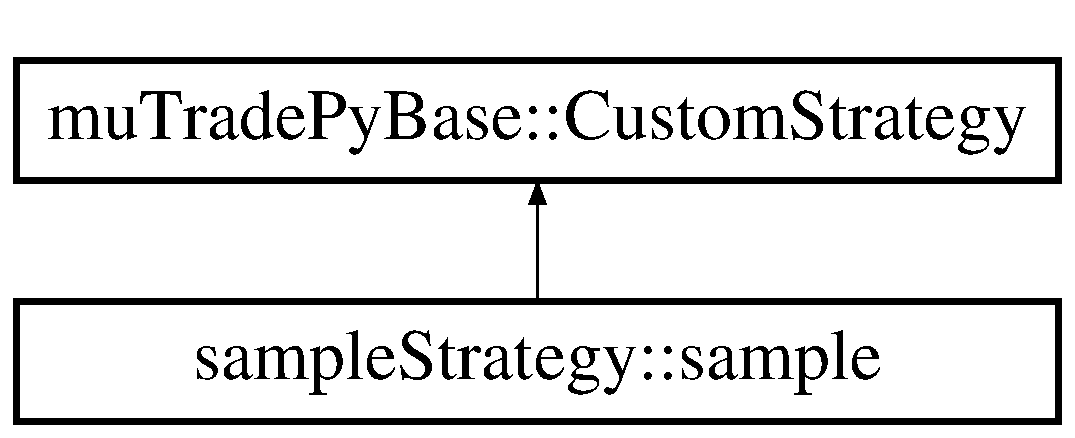
\includegraphics[height=2.000000cm]{classsampleStrategy_1_1sample}
\end{center}
\end{figure}
\subsection*{Public Member Functions}
\begin{DoxyCompactItemize}
\item 
\hypertarget{classsampleStrategy_1_1sample_a824adf637925f01e6e95a68695e0a8df}{def {\bfseries \-\_\-\-\_\-init\-\_\-\-\_\-}}\label{classsampleStrategy_1_1sample_a824adf637925f01e6e95a68695e0a8df}

\item 
\hypertarget{classsampleStrategy_1_1sample_a0276042f0a48f1b13bb24d7c5a980f6a}{def {\bfseries on\-Init\-Event}}\label{classsampleStrategy_1_1sample_a0276042f0a48f1b13bb24d7c5a980f6a}

\item 
\hypertarget{classsampleStrategy_1_1sample_ae189229b773474fc8b01e519a3d1a354}{def {\bfseries on\-C\-M\-D\-Modify\-Strategy}}\label{classsampleStrategy_1_1sample_ae189229b773474fc8b01e519a3d1a354}

\item 
\hypertarget{classsampleStrategy_1_1sample_a8772d8f9aecaf9e7fb9f9a0aa087435d}{def {\bfseries on\-C\-M\-D\-Terminate\-Startegy}}\label{classsampleStrategy_1_1sample_a8772d8f9aecaf9e7fb9f9a0aa087435d}

\item 
\hypertarget{classsampleStrategy_1_1sample_ad24fe84a685be8bf30434275ff46700c}{def {\bfseries on\-C\-M\-D\-Terminate\-Sq\-Off\-Strategy}}\label{classsampleStrategy_1_1sample_ad24fe84a685be8bf30434275ff46700c}

\item 
\hypertarget{classsampleStrategy_1_1sample_a837817933dcbaa2bcf6c6d79a7f99a0d}{def {\bfseries on\-Market\-Data\-Event}}\label{classsampleStrategy_1_1sample_a837817933dcbaa2bcf6c6d79a7f99a0d}

\item 
\hypertarget{classsampleStrategy_1_1sample_a2d63e2ced58bf5712c1e6f7e85cf5cf5}{def {\bfseries on\-Ohlc\-Time\-Out\-Event}}\label{classsampleStrategy_1_1sample_a2d63e2ced58bf5712c1e6f7e85cf5cf5}

\item 
\hypertarget{classsampleStrategy_1_1sample_a80d7ffc2501684bf05ffb5f436eb106b}{def {\bfseries on\-Confirmed}}\label{classsampleStrategy_1_1sample_a80d7ffc2501684bf05ffb5f436eb106b}

\item 
\hypertarget{classsampleStrategy_1_1sample_a40b6a062417472d03b4631b7a27916f4}{def {\bfseries on\-Replaced}}\label{classsampleStrategy_1_1sample_a40b6a062417472d03b4631b7a27916f4}

\item 
\hypertarget{classsampleStrategy_1_1sample_a1cc4858996ea43ac462f030b6720088e}{def {\bfseries on\-Replace\-Rejected}}\label{classsampleStrategy_1_1sample_a1cc4858996ea43ac462f030b6720088e}

\item 
\hypertarget{classsampleStrategy_1_1sample_aa3d18273289d513d6abe5fc04a67b751}{def {\bfseries on\-Cancel\-Rejected}}\label{classsampleStrategy_1_1sample_aa3d18273289d513d6abe5fc04a67b751}

\item 
\hypertarget{classsampleStrategy_1_1sample_adaccfc4c93c1246ba20206f37d2052c3}{def {\bfseries on\-New\-Rejected}}\label{classsampleStrategy_1_1sample_adaccfc4c93c1246ba20206f37d2052c3}

\item 
\hypertarget{classsampleStrategy_1_1sample_a488f5f86c3fb036432f01d6f6f37cb83}{def {\bfseries on\-I\-O\-C\-Cancelled}}\label{classsampleStrategy_1_1sample_a488f5f86c3fb036432f01d6f6f37cb83}

\item 
\hypertarget{classsampleStrategy_1_1sample_a7e4f23b6fa39aba0065c268913b98ef3}{def {\bfseries on\-Filled}}\label{classsampleStrategy_1_1sample_a7e4f23b6fa39aba0065c268913b98ef3}

\item 
\hypertarget{classsampleStrategy_1_1sample_a167412a5ffdc877b00ab0273eb773099}{def {\bfseries on\-Partial\-Fill}}\label{classsampleStrategy_1_1sample_a167412a5ffdc877b00ab0273eb773099}

\item 
\hypertarget{classsampleStrategy_1_1sample_a1f1606ccf7f97d7b969c7a00a5d95793}{def {\bfseries on\-Market\-To\-Limit}}\label{classsampleStrategy_1_1sample_a1f1606ccf7f97d7b969c7a00a5d95793}

\item 
\hypertarget{classsampleStrategy_1_1sample_a4337acef57f06773fdd1c5cc09d40441}{def {\bfseries on\-Frozen}}\label{classsampleStrategy_1_1sample_a4337acef57f06773fdd1c5cc09d40441}

\item 
\hypertarget{classsampleStrategy_1_1sample_a3a5c986bc3d0eb22af8fe51c02c37c22}{def {\bfseries on\-Timer\-Event}}\label{classsampleStrategy_1_1sample_a3a5c986bc3d0eb22af8fe51c02c37c22}

\end{DoxyCompactItemize}
\subsection*{Public Attributes}
\begin{DoxyCompactItemize}
\item 
\hypertarget{classsampleStrategy_1_1sample_a918c4c9d2bbf76d992818bbb9e560aa4}{{\bfseries f}}\label{classsampleStrategy_1_1sample_a918c4c9d2bbf76d992818bbb9e560aa4}

\item 
\hypertarget{classsampleStrategy_1_1sample_a6d2312273f20c1c5a07373b253e5e64d}{{\bfseries Trade\-Instrument}}\label{classsampleStrategy_1_1sample_a6d2312273f20c1c5a07373b253e5e64d}

\end{DoxyCompactItemize}


The documentation for this class was generated from the following file\-:\begin{DoxyCompactItemize}
\item 
sample\-Strategy.\-py\end{DoxyCompactItemize}

\chapter{File Documentation}
\hypertarget{muTradePyBase_8py}{
\section{muTradePyBase.py File Reference}
\label{muTradePyBase_8py}\index{muTradePyBase.py@{muTradePyBase.py}}
}
\subsection*{Classes}
\begin{DoxyCompactItemize}
\item 
class \hyperlink{classmuTradePyBase_1_1CustomStrategy}{muTradePyBase::CustomStrategy}
\end{DoxyCompactItemize}
\subsection*{Namespaces}
\begin{DoxyCompactItemize}
\item 
namespace \hyperlink{namespacemuTradePyBase}{muTradePyBase}
\end{DoxyCompactItemize}

\hypertarget{README_8md}{
\section{README.md File Reference}
\label{README_8md}\index{README.md@{README.md}}
}

\hypertarget{sampleStrategy_8py}{
\section{sampleStrategy.py File Reference}
\label{sampleStrategy_8py}\index{sampleStrategy.py@{sampleStrategy.py}}
}
\subsection*{Classes}
\begin{DoxyCompactItemize}
\item 
class \hyperlink{classsampleStrategy_1_1sample}{sampleStrategy::sample}
\end{DoxyCompactItemize}
\subsection*{Namespaces}
\begin{DoxyCompactItemize}
\item 
namespace \hyperlink{namespacesampleStrategy}{sampleStrategy}
\end{DoxyCompactItemize}

\printindex
\end{document}
